%% Manuscript prepared with the official MDPI LaTeX template (journal: Healthcare).
%% Class, .bst and logos are the genuine MDPI template files in ./Definitions/.
%% Healthcare 임상정보학 맥락과 Methods/Results 수치는 이 폴더의
%% results/run_crosscorpus*.txt 및 revision_* 근거 원장에 맞춰 통합했다.

\documentclass[healthcare,article,submit,moreauthors,pdftex]{Definitions/mdpi}
\renewcommand{\today}{July 27, 2026}

\usepackage{amssymb}
\usepackage{array}
\newcolumntype{L}[1]{>{\raggedright\arraybackslash}p{#1}}

% ------------------------------------------------------------------ front matter
\firstpage{1}
\makeatletter
\setcounter{page}{1}
\makeatother
\pubvolume{1}
\issuenum{1}
\articlenumber{0}
\pubyear{2026}
\copyrightyear{2026}
\history{Received: ; Revised: ; Accepted: ; Published: }

\Title{When Wellness Stress Detection Enters Healthcare Workflows: An
Iso-Heart-Rate, Cross-Corpus Evaluation of Wrist Wearables}

% ORCID: mdpi.cls turns \orcidA{} into a linked ORCID icon using \orcidauthorA.
\newcommand{\orcidauthorA}{0000-0002-5072-3632}
\Author{Nowon Kwon $^{1}$\orcidA{}, Seonkyung Yoon $^{2}$, Jungyi Hur $^{2}$ and Hye Seung Kang $^{2,}$*}
\AuthorNames{Nowon Kwon, Seonkyung Yoon, Jungyi Hur and Hye Seung Kang}

\address{%
$^{1}$ \quad AI-driven Medical Innovation Center, Kyungpook National University Hospital, Daegu 41944, Republic of Korea\\
$^{2}$ \quad Department of Nursing, Saekyung University, Yeongwol 26239, Republic of Korea}

\corres{Correspondence: hskang3164@saekyung.ac.kr}

\abstract{\textbf{Background/Objectives:} Benchmark performance does not establish that a
wrist-wearable stress measure is valid in healthcare workflows. We tested whether
binary stress-versus-non-stress performance reflects stress-specific physiology
rather than heart-rate (HR) arousal, and whether models generalize from
wellness-like corpora to a clinical workforce context.
\textbf{Methods:} We analyzed three public wrist Empatica~E4 corpora: WESAD,
Stress-Predict, and a real-world Nurse dataset. An iso-heart-rate (iso-HR)
evaluation balanced HR within subject before measuring non-cardiac
discriminability. We compared a continuous skin
conductance response (SCR) count with logistic regression, gradient boosting,
four unsupervised domain-adaptation methods, and an accelerometer context-aware
variant, under leave-one-subject-out and leave-one-dataset-out evaluation with
subject-cluster bootstrap intervals. \textbf{Results:} The single SCR score was
statistically indistinguishable from logistic regression in paired cross-corpus
tests, and no adaptation method moved a weak corpus into a usable range: across
all evaluated models transfer AUROC was approximately 0.90 with WESAD as target
but 0.52--0.57 with Stress-Predict or Nurse. Adding activity context raised
within-corpus AUROC yet lowered cross-corpus transfer, because the
movement--stress association reverses across protocols. On Nurse, source-trained
models reached AUROC 0.541--0.559 against prevalence 0.796 with poor calibration,
and conditioning on movement or on distance to the source distribution removed the
residual discrimination. Iso-HR evidence was diagnostic mainly in WESAD. \textbf{Conclusions:} Neither shallow
unsupervised adaptation nor wrist activity context established reliable transfer
to Nurse, and sparse retrospective labels prevent attributing this solely to
physiological non-transfer. Cross-corpus and iso-HR controls, not model
complexity, determine what can be concluded for healthcare workflows.}

\keyword{digital health; Healthcare; wearable sensors; nursing workforce;
electrodermal activity; stress detection; heart-rate confounding; clinical
informatics; domain generalization; alert fatigue}

\begin{document}

% =====================================================================
\section{Introduction}
% =====================================================================

Wearable biosensors and affective computing have made continuous physiological
stress monitoring increasingly visible in digital health, public health, and
occupational wellness. Wrist-worn devices such as the Empatica~E4 and consumer
smartwatches can collect autonomic signals unobtrusively during daily life,
including heart rate (HR), heart-rate variability (HRV), electrodermal activity
(EDA), and skin temperature~\cite{can2019survey,schmidt2019review}. Motivated by
this technological promise, machine-learning studies have optimized stress
classification pipelines on laboratory datasets, often reporting binary
stress-detection performance around or above 90\% in controlled experimental
designs~\cite{schmidt2018wesad,gjoreski2017wrist,siirtola2020}. These results
have helped establish wearable stress detection as a plausible digital health
application, and related Healthcare studies have examined wearable stress
management and context-aware smart-band feedback in real-life
settings~\cite{gonzalezramirez2023wearablesstress,can2020relax}.

Yet a digital health signal becomes clinically meaningful only after its context
of use has been specified and its measurement validity has been established.
Digital medicine frameworks distinguish technical verification, analytical
validation, and clinical validation, and emphasize that biometric monitoring
technologies should be fit for the intended population and setting before their
outputs are interpreted as health measures~\cite{goldsack2020v3}. Similarly,
patient- and user-centered digital-measure frameworks caution against
proliferating low-value measures that are technically measurable but burdensome or
weakly connected to decisions that matter in care~\cite{manta2020digitalmeasures}.
For stress monitoring, this distinction is central: a wearable score that is
acceptable as a private wellness cue may be inappropriate as an input to clinical
workflow, staffing, or occupational-health decisions.

For healthcare context-of-use validation, however, the relevant question is not only
whether a model can classify stress within a familiar benchmark. The harder
question is whether a model trained under wellness or laboratory conditions
remains valid when it is moved into an active clinical workforce. These concerns
are especially salient in safety-critical and emotionally intensive occupations,
where stress monitoring is not merely a private wellness function but may become
linked to work design, occupational health, staffing, care quality, or patient
safety. Frontline healthcare work is a clear example. The COVID-19 context made
psychological strain among healthcare workers highly visible~\cite{lai2020mentalhealth,
sasangohar2020provider}, and nursing stress and burnout drew particular attention
because their implications extend beyond individual well-being to workload,
workforce retention, care quality, and patient safety~\cite{dallora2020burnout,
hall2016staffwellbeing}. At the same time, clinical work is physiologically
complex: cognitive-emotional strain occurs alongside walking, lifting, shift
work, alarms, interruptions, and urgent bedside
tasks~\cite{hosseini2022nurse,ruppel2023alarmburden,gulsen2025alarmfatigue}.
Nursing is therefore a useful boundary case for wrist-wearable stress detection,
not because this study seeks a nurse-specific predictor, but because it provides
a demanding context-of-use test in which a wellness stress score may lose
validity.

This translational risk is amplified by a physiological confound. Stress tasks
often elevate HR, but HR is not specific to psychological stress. Physical
activity, posture, thermoregulation, and routine clinical work can also increase
HR and alter wrist physiology~\cite{kreibig2010ans,boucsein2012eda}. A wearable
classifier may therefore achieve high apparent performance by separating
high-arousal movement from low-arousal rest, rather than detecting
stress-specific physiology. In a hospital ward, this distinction matters: a model
that mistakes patient lifting or urgent movement for psychological strain may
generate operational noise rather than protective insight. Thus, before consumer
smartwatch stress scores or wellness stress dashboards are scaled into healthcare
workforce monitoring or organizational wellness programs, their physiological
boundary conditions need to be tested
explicitly~\cite{virgillito2025wearablesorg}.

A second barrier is cross-corpus generalizability. Even leave-one-subject-out
validation within one dataset evaluates new people under the same stressor type,
device configuration, labeling scheme, and preprocessing assumptions. It does not
establish that models trained on laboratory social-evaluative stress or mild
cognitive stress will transfer to naturalistic hospital work. This evolution is
also reflected in the public datasets available for wrist-based stress research.
Controlled corpora such as WESAD support benchmark development, whereas more
naturalistic datasets test whether stress models survive changes in stressor
type, activity context, and labeling conditions. Recent work has emphasized that
stressor type can dominate cross-dataset generalizability in physiological stress
detection~\cite{prajod2024}. Systematic reviews likewise identify limited
statistical power, inconsistent labeling, and weak evidence for generalization as
recurring problems in wearable stress research~\cite{vos2023generalizable}.
Recent studies have begun to address this gap using real-life ecological
momentary assessment (EMA) designs, office-like work simulations, cross-dataset
HRV analyses, and cross-context/domain-adaptation
frameworks~\cite{tutunji2023prolonged,naegelin2023interpretable,
benchekroun2023crossdataset,mihirette2025crosscontextual}. New datasets that
explicitly combine acute stress and exercise further show why physical arousal
must be handled as a competing context rather than a nuisance
variable~\cite{hongn2025wearable}. From a Healthcare perspective, the Nurse
corpus should therefore not be treated simply as a difficult or low-performing
dataset. It is an ecologically demanding test of whether models trained or
validated in wellness-like conditions retain meaning in clinical workforce
settings.

In this study we use three public wrist Empatica~E4 corpora to define these
boundaries: Wearable Stress and Affect Detection (WESAD), Stress-Predict, and a
real-world Nurse dataset collected from hospital
nurses~\cite{schmidt2018wesad,talukdar2022stresspredict,hosseini2022nurse}. We
do not propose a new deployable stress monitor. Instead, we ask three
translational questions. \textbf{(RQ1)} Does multivariate machine learning
provide reliable value beyond a single interpretable skin conductance response
(SCR) feature?
\textbf{(RQ2)} Does stress-detection performance transfer across stressor types
and into the Nurse corpus? \textbf{(RQ3)} Does HR-level confounding explain the
observed corpus differences, and in which corpora is an iso-HR decomposition
diagnostic? To
answer these questions, we introduce an iso-heart-rate (iso-HR) evaluation that
balances HR within subject before measuring the residual discriminability of
non-cardiac signals. The purpose is to turn laboratory-to-clinic generalization
into a measurable validity problem: before wearable stress outputs are treated as
actionable in healthcare workflows, they should survive HR control and
cross-corpus testing.

% =====================================================================
\section{Materials and Methods}
% =====================================================================

\subsection{Analysis Overview}

The analysis was designed to make the translation problem visible rather than to
maximize a single benchmark score. Figure~\ref{fig:workflow} shows the
context-of-use validation workflow, and Table~\ref{tab:pipeline} summarizes the
full pipeline from public datasets to clinically oriented interpretation.

\begin{figure}[H]
\centering
\resizebox{0.96\textwidth}{!}{%
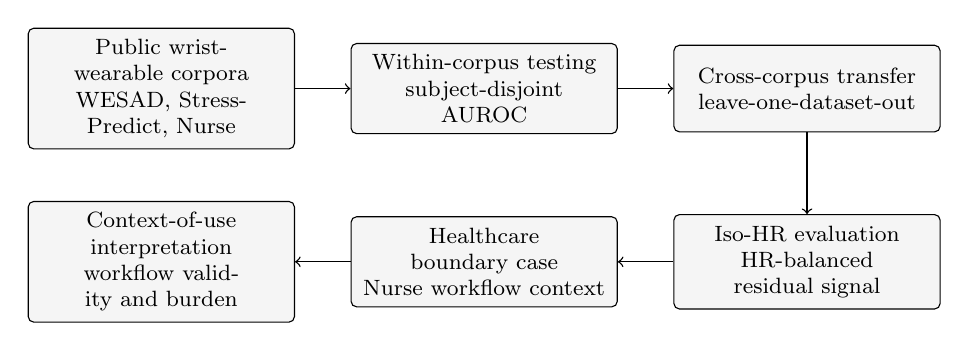
\begin{tikzpicture}[
box/.style={draw, rounded corners=2pt, fill=gray!8, align=center,
font=\footnotesize, text width=3.1cm, minimum height=1.1cm, inner sep=4pt},
arrow/.style={->, line width=0.5pt}
]
\node[box] (data) at (0,0) {Public wrist-wearable corpora\\WESAD, Stress-Predict, Nurse};
\node[box] (within) at (4.1,0) {Within-corpus testing\\subject-disjoint AUROC};
\node[box] (transfer) at (8.2,0) {Cross-corpus transfer\\leave-one-dataset-out};
\node[box] (isohr) at (8.2,-2.2) {Iso-HR evaluation\\HR-balanced residual signal};
\node[box] (boundary) at (4.1,-2.2) {Healthcare boundary case\\Nurse workflow context};
\node[box] (interpret) at (0,-2.2) {Context-of-use interpretation\\workflow validity and burden};
\draw[arrow] (data) -- (within);
\draw[arrow] (within) -- (transfer);
\draw[arrow] (transfer) -- (isohr);
\draw[arrow] (isohr) -- (boundary);
\draw[arrow] (boundary) -- (interpret);
\end{tikzpicture}}
\caption{Context-of-use validation workflow for wearable stress classification.
The workflow separates benchmark performance from healthcare translation by
adding cross-corpus transfer, HR control, and workflow-sensitive interpretation
before considering clinical workforce use.\label{fig:workflow}}
\end{figure}

\begin{table}[H]
\centering
\caption{Analysis pipeline and design rationale.\label{tab:pipeline}}
\begin{tabular}{p{0.20\textwidth}p{0.72\textwidth}}
\toprule
\textbf{Step} & \textbf{Purpose and implementation} \\
\midrule
Data sources &
Use three public Empatica~E4 corpora spanning laboratory social-evaluative stress
(WESAD), mild cognitive stress (Stress-Predict), and real-world hospital nurse
work (Nurse). \\
Windowing &
Segment wrist signals into 64~s windows with 50\% overlap to obtain comparable
physiological epochs across corpora. \\
Signal processing &
Extract HR/HRV, EDA, temperature, and accelerometer-derived quantities; decompose
EDA into tonic and phasic components and count SCR events. \\
Feature design &
Compare one fixed, interpretable SCR feature against multivariate logistic
regression, histogram gradient boosting, and correlation alignment (CORAL). \\
Transfer control &
Use subject-disjoint validation within corpora and leave-one-dataset-out testing
across corpora to distinguish benchmark performance from translation. \\
HR-confound control &
Apply iso-HR matching within subject, then compare all-feature, HR-level-free, and
non-cardiac feature sets using the HR-leakage index. \\
Uncertainty &
Report subject-cluster bootstrap intervals, paired subject-bootstrap model
differences, and cluster-aware permutation tests. \\
Healthcare interpretation &
Interpret weak Nurse-corpus transfer as a workflow-validity warning while
separating physiological non-transfer from sparse, retrospective ground-truth
limitations. \\
\bottomrule
\end{tabular}
\end{table}

\subsection{Datasets}

We use three publicly available wrist Empatica~E4 corpora
(Table~\ref{tab:corpora}). \textbf{WESAD}~\cite{schmidt2018wesad} provides
laboratory social-evaluative stress (Trier Social Stress Test,
TSST~\cite{kirschbaum1993tsst}) versus baseline/meditation. \textbf{Stress-Predict}
\cite{talukdar2022stresspredict} provides mild cognitive stress (Stroop task and
a mock interview) versus relaxation, which we label from the published protocol
time-logs rather than from a precomputed label column. \textbf{Nurse}
\cite{hosseini2022nurse} provides real-world hospital recordings with
retrospective self-reported stress levels (we contrast the survey extremes,
high-stress vs.\ no-stress, excluding the ambiguous middle level). From each
corpus we form a binary stress(+)/non-stress($-$) task using the wrist E4 streams
(blood-volume pulse 64~Hz, EDA 4~Hz, skin temperature 4~Hz, accelerometer
32~Hz); device characteristics are as validated previously~\cite{mccarthy2016e4}.

\begin{table}[H]
\centering
\caption{Cross-corpus evaluation datasets (wrist Empatica~E4).\label{tab:corpora}}
\begin{tabular}{lrrrl}
\toprule
\textbf{Corpus} & \textbf{Windows} & \textbf{$+/-$} & \textbf{Subjects} & \textbf{Stressor} \\
\midrule
WESAD          & 1{,}133 & 287/846        & 15 & TSST (social-evaluative) \\
Stress-Predict & 2{,}846 & 952/1{,}894    & 35 & Stroop + mock interview (cognitive) \\
Nurse          & 9{,}226 & 7{,}347/1{,}879 & 15 & Real-world hospital (self-report) \\
\bottomrule
\end{tabular}
\end{table}

\subsection{Operational Definition of Healthcare Context-of-Use}

For this analysis, healthcare context-of-use is defined as the condition in
which a wearable stress output would be interpreted within an active clinical
workforce workflow rather than as a private wellness reflection. This definition
has three components. First, the signal must retain meaning under the physical
conditions of care work, including walking, standing, lifting, urgent movement,
thermal variation, and device-fit changes during long shifts. Second, the signal
must remain interpretable under cognitive and emotional conditions that differ
from laboratory stressors, such as alarms, interruptions, multitasking, time
pressure, patient deterioration, and interpersonal conflict. Third, the output
must have a plausible action pathway: it may enter a dashboard, alert, staffing
conversation, occupational-health review, or well-being intervention. These
requirements make healthcare context-of-use stricter than ordinary
within-dataset classification, because errors do not merely reduce an AUROC
score; they can add workflow noise, staff concern, or misleading operational
interpretation.

The three corpora are therefore not treated as interchangeable samples from one
stress population. Instead, they operationalize three increasingly demanding
context-of-use conditions for a wrist-based stress measure. WESAD represents
benchmark validity: whether wrist physiology can detect a strong,
protocol-defined social-evaluative stressor. Stress-Predict represents
stressor-shift validity: whether a model or feature remains useful when the
stressor is milder and more cognitive. The Nurse corpus represents healthcare
workflow validity: whether a wellness-like stress output retains meaning when
physiological arousal is embedded in real clinical work and retrospective
self-report. Under this operational definition, the Nurse corpus is not included
because the study aims to build a nurse-specific predictor. It is included
because it is a boundary case for healthcare translation. Table~\ref{tab:contextdefinition}
states this role explicitly.

\begin{table}[H]
\centering
\caption{Operational role of each corpus in the context-of-use analysis.\label{tab:contextdefinition}}
\begin{tabular}{@{}L{0.13\textwidth}L{0.25\textwidth}L{0.31\textwidth}L{0.23\textwidth}@{}}
\toprule
\textbf{Corpus} & \textbf{Operational context} & \textbf{Validity question} & \textbf{Interpretation of failure} \\
\midrule
WESAD &
Controlled social-evaluative laboratory stress. &
Can wrist physiology classify a strong, protocol-defined stressor under
benchmark conditions? &
Weak performance would challenge the basic physiological signal. \\
Stress-Predict &
Milder cognitive and interview stress in a structured protocol. &
Does the signal survive a shift in stressor type and labeling protocol? &
Weak performance suggests stressor-dependent physiology or label-alignment
limits. \\
Nurse &
Naturalistic hospital work with movement, interruptions, alarms, shift demands,
and retrospective self-report. &
Does a wellness-like wearable stress measure retain meaning in a healthcare
workforce workflow? &
Weak performance indicates unsupported healthcare translation without richer
context, not a nurse-specific model failure. \\
\bottomrule
\end{tabular}
\end{table}

\subsection{Windowing and Features}
\label{sec:features}

Signals are segmented into 64~s windows with 50\% overlap. EDA is decomposed into
tonic and phasic components with cvxEDA~\cite{greco2016cvxeda} as implemented in
NeuroKit2~\cite{makowski2021neurokit}; skin-conductance responses (SCRs) are
counted as local maxima of the phasic signal~\cite{benedek2010phasic}. From each
window we compute four feature families: (i)~\emph{HR level} (mean HR, mean
inter-beat interval [IBI]); (ii)~\emph{cardiac dynamics/variability}: HR slope, range
and curvature, and HRV indices (RMSSD, SDNN, pNN50, with a Malik-rule artifact
flag)~\cite{shaffer2017hrv}; (iii)~\emph{non-cardiac}: tonic and phasic EDA
(SCR count, amplitude, area, decay) and skin temperature (mean, slope); and
(iv)~\emph{activity/movement}, derived from the 32~Hz three-axis wrist
accelerometer as the vector-magnitude mean, standard deviation, Euclidean norm
minus one, and mean absolute jerk. All three corpora record wrist accelerometry
on the same Empatica scale, so the activity block is computed identically in
each. Families (i)--(iii) enter the classification models; family~(iv) is used
for the movement stratification (Section~\ref{sec:isohr}) and for the
context-aware model described below, and never enters the primary feature set.
The
single most discriminative EDA feature in within-fold permutation importance is
the SCR count, which we use as the single-feature predictor. It is therefore the
best single EDA feature selected within training folds rather than an unexamined
a priori feature choice. Its decision
direction is fixed \emph{a priori} (more SCRs $\rightarrow$ more stress); it is
never flipped using test labels, so a below-chance area under the receiver
operating characteristic curve (AUROC) is reported as such. SCR count remains a
continuous score for the primary AUROC analysis, so no classification threshold
is selected. For robustness, we repeat the full protocol with non-overlapping
64~s windows (64~s step) and with 300~s windows at 50\% overlap (150~s step).
At both window lengths we also compare otherwise identical all-feature models
with models omitting six HRV/quality variables: RMSSD, SDNN, pNN50, valid-IBI
count, IBI coefficient of variation, and artifact fraction. For
cross-corpus transfer we additionally restrict to a \emph{transfer-robust} set of
eight device- and ambient-invariant quantities: phasic SCR count, mean and
maximum SCR amplitude, phasic area, tonic (skin-conductance-level) slope, EDA
decay, temperature slope, and HR slope. Absolute means (mean HR, mean skin
conductance, mean temperature) are excluded because they do not transfer across
devices. The context-aware variant evaluated in Section~\ref{sec:context}
appends the four activity features to these eight, giving twelve inputs.

\subsection{Iso-HR Matching and the HR-leakage Index}

To separate stress-specific physiology from non-specific arousal, we balance HR
before evaluation. Within each subject, windows are binned into 5~bpm HR bins and
the majority class is randomly subsampled so that the two classes have identical
HR distributions per bin. This iso-HR matched set is a study-design subsampling
that uses HR and labels only to balance counts and \emph{never} participates in
model fitting. Because the subsample is random, the matching is repeated over
multiple seeds and we report the stability of the resulting estimates
(Section~\ref{sec:isohr}).

Operationally, matching is performed on whole precomputed windows, separately
for each subject:
\begin{enumerate}
\item assign every intact window to a 5~bpm bin using its mean HR;
\item within each subject--bin combination, set the retained count to the
smaller of the stress and non-stress counts;
\item sample that number of complete windows from each class without removing
or splicing any signal samples; and
\item concatenate the retained windows and perform subject-wise evaluation.
\end{enumerate}
Bins containing only one class contribute no windows. Features, including HRV,
are not recomputed after matching because the unit of selection is the intact
window. This procedure can remove many windows when within-subject class overlap
in HR is limited; we therefore report matched sample sizes and seven-seed
stability.

On the matched set we evaluate three nested feature sets: \emph{all features}
(including HR level); \emph{HR-level-free} (all features \emph{except} mean HR and
mean IBI; this still contains cardiac dynamics and HRV, so it is not
``non-cardiac''); and \emph{non-cardiac} (EDA and temperature only). We define the
\emph{HR-leakage index} as the matched-set AUROC of the all-feature model minus
that of the HR-level-free model; a value near zero means that HR \emph{level}
contributes little once the other signals are present. We emphasize that a
near-zero index is informative only where a discriminative signal exists at all;
in a corpus where every feature set is near chance, the index is near zero
trivially (a floor effect) and carries no evidence about confounding.

\subsection{Models and Evaluation}

We compare two groups of predictors, plus two further variants defined below. The \emph{reference} group contains
(i)~a \emph{single feature}, the SCR count used directly as a score with no
training, which makes it \emph{corpus-invariant by construction}: its
within-corpus and cross-corpus AUROC on a given target are identical because
nothing is fit; (ii)~\emph{logistic regression} (linear; per-fold median
imputation and standardization fit on training data only); and
(iii)~\emph{histogram gradient boosting} (non-linear, with native missing-value
handling).

The \emph{unsupervised adaptation} group contains four methods that see the
target's feature distribution but never its labels:
\emph{CORAL}~\cite{sun2016coral}, which aligns second-order statistics of the
source to those of the target; \emph{subspace alignment}~\cite{fernando2013subspace},
which maps the source principal axes onto the target principal axes;
\emph{transfer component analysis}~\cite{pan2011tca}, which learns a kernel
subspace minimizing the maximum mean discrepancy between domains; and
\emph{importance-weighted logistic regression}, which reweights source windows by
a domain-classifier density ratio to correct covariate
shift~\cite{shimodaira2000covariateshift,sugiyama2008importance,bickel2009discriminative}. All four are
transductive: they use the \emph{unlabeled} target feature distribution, which
the reference models never see, so their failure to beat those models is a
conservative result. Subspace alignment and transfer component analysis require hyperparameters for
which no a-priori rule exists. We therefore sweep them and report the setting that
\emph{maximizes target AUROC}: 2--8 components for subspace alignment, and the
same component range crossed with three RBF bandwidths ($0.5\times$, $1\times$
and $2\times$ the median-distance heuristic) for transfer component analysis,
because both conventions appear in the literature and the result is sensitive to
the choice. Each reported value is therefore an optimistic upper bound that no
honest selection rule can exceed, so a conclusion that survives it does not depend
on hyperparameter selection.
Transfer component analysis is fitted on a fixed-seed subsample of 1{,}000
windows per domain because a full kernel eigendecomposition over all windows is
not tractable; the learned map is then applied to every window.

The \emph{context-aware} variant (Section~\ref{sec:context}) appends the four
wrist-accelerometer activity features to the eight transfer features and is
otherwise identical to logistic regression and gradient boosting. To separate
adaptation limits from target-signal limits, we additionally report a
\emph{supervised} reference in which $k \in \{2,4,8\}$ target subjects are
labeled and added to the training set, with evaluation on the remaining target
subjects over 20 fixed-seed draws; this is not leave-one-dataset-out and is
reported separately as an upper bound. Within-corpus performance uses
leave-one-subject-out (LOSO) cross-validation; cross-corpus generalization uses
\emph{leave-one-dataset-out} (train on the union of the other corpora, test on
the held-out corpus). AUROC is the primary metric. For leave-one-dataset-out
target estimates and paired model differences, uncertainty is estimated by a
subject-level cluster bootstrap (1{,}000 resamples)~\cite{efron1993bootstrap};
the within-corpus LOSO table reports point estimates. Significance against chance
is assessed by a cluster-aware permutation test that retains the fixed target
scores and subject set, shuffles labels \emph{within} each subject, and
recomputes the statistic. This preserves subject structure and class balance;
$p$-values across the family of cross-corpus tests are Holm-corrected.
The two procedures answer different questions: the bootstrap quantifies
generalization to \emph{new subjects}, whereas the within-subject permutation,
which holds the subject set fixed, tests only whether a within-corpus association
exceeds chance. We therefore treat the subject-cluster bootstrap as the primary,
more conservative summary for generalization claims and use the permutation as a
secondary check. To compare \emph{models} (rather than against chance), we use a
paired subject-cluster bootstrap of the AUROC difference and call two models
statistically indistinguishable when the 95\% interval of their difference
contains zero.

For the imbalanced Nurse target we additionally report average precision, Brier
score, 10-bin expected calibration error (ECE), balanced accuracy, sensitivity,
and false-positive rate (FPR). Logistic-regression and boosting operating
metrics use a fixed probability threshold of 0.5 chosen before inspecting Nurse
labels; it is not tuned on the target. To describe, rather than causally explain,
domain discrepancy, each transfer feature is compared between corpus pairs using
one-dimensional Wasserstein distance divided by the pairwise pooled interquartile
range. Stress-Predict label alignment is assessed by shifting all protocol
intervals by $-64$, $-32$, 0, $+32$, and $+64$~s while keeping every other
analysis choice fixed.

\subsection{Reproducibility and Leakage Control}

The only train/test partition is by subject; subjects never appear on both sides
(enforced by an assertion, with split sessions merged so one subject cannot enter
both folds). Iso-HR matching never fits a model, and gradient boosting handles
missing values natively, so no scaler or imputer statistics leak from training to
test. We ran an adversarial code review for cross-subject leakage and found none;
a within-subject look-ahead remains because EDA decomposition is computed once per
session, but this is not a cross-subject leak and does not inflate LOSO estimates.
As a negative control we permuted labels \emph{within} each subject, preserving
every subject's class balance, and re-ran the whole within-corpus pipeline
unchanged over five permutations. It returns AUROC $0.482 \pm 0.023$ on WESAD and
$0.481 \pm 0.019$ on Stress-Predict, so no label information reaches the model
through feature construction, the split, or the evaluation path. On Nurse the
same control returns $0.298 \pm 0.011$. A below-chance value cannot indicate
leakage, which would inflate rather than deflate the statistic; it reflects the
fact that pooled Nurse AUROC is governed by between-subject score offsets against
strongly unequal per-subject prevalences---the same structure that
Section~\ref{sec:errstrata} isolates by conditioning. All bootstrap resampling
is by subject and all permutations remain within subject, so overlapping windows
never cross train/test or resampling blocks. Analyses used Python 3.11.13 with
scikit-learn 1.9.0, NumPy 2.4.6, SciPy 1.17.1, pandas 2.3.3, NeuroKit2 0.2.13 and
CVXOPT 1.3.3; the complete environment, with exact pins for every dependency, is
specified in \texttt{env.yaml}. All supported commands run through versioned
shell entry points in \texttt{scripts/}, and all randomness uses fixed, reported
seeds. Analysis code is prepared for public release (Data Availability
Statement).

% =====================================================================
\section{Results}
% =====================================================================

\subsection{A Single Skin-Conductance Feature Is on Par with Machine Learning}

Within each corpus (Table~\ref{tab:within}; feature families and the
transfer-robust set are defined in Section~\ref{sec:features}), a single SCR
feature is on par with
linear and non-linear machine learning where the signal is strong: on WESAD it
reaches AUROC $0.897$ versus $0.876$ (logistic) and $0.886$ (boosting). Machine
learning shows a modest edge only on the mild-cognitive corpus (Stress-Predict,
$0.628$/$0.633$ vs.\ $0.563$, $\Delta\approx0.07$), where \emph{all} models
nonetheless remain weak ($<0.65$); on the real-world corpus (Nurse) every model
is near chance and the single feature ($0.553$) is not beaten by logistic
regression ($0.450$, i.e., below chance under LOSO, indicating subject-level
heterogeneity rather than learnable structure). Thus added model capacity yields
no consistent advantage over the single interpretable feature; where it appears
to help, the absolute performance is still too low to be clinically useful. This
points to a univariate physiological effect rather than a machine-learning
achievement.

\begin{table}[H]
\centering
\caption{Within-corpus leave-one-subject-out AUROC. A single skin-conductance
feature is on par with machine learning where the signal is strong (WESAD);
machine learning shows only a modest edge on the mild-cognitive corpus
(Stress-Predict), where all models remain weak. Values are LOSO point estimates;
uncertainty for the transfer claims is given in Table~\ref{tab:lodo}.\label{tab:within}}
\begin{tabular}{lccc}
\toprule
\textbf{Within-corpus (LOSO)} & \textbf{Single (SCR)} & \textbf{Logistic} & \textbf{Gradient boosting} \\
\midrule
WESAD          & \textbf{0.897} & 0.876 & 0.886 \\
Stress-Predict & 0.563 & 0.628 & 0.633 \\
Nurse          & 0.553 & 0.450 & 0.489 \\
\bottomrule
\end{tabular}
\end{table}

\subsection{Cross-Corpus Transfer Is Poor for Every Model Evaluated}

Leave-one-dataset-out transfer (Table~\ref{tab:lodo}, Figure~\ref{fig:f1}) is
strong only when the target corpus is WESAD and weak otherwise. The single feature
is corpus-invariant by construction, so its $0.897$ on WESAD is identical to its
within-corpus value; notably, the logistic model trained on the \emph{other}
corpora also transfers to WESAD almost as well ($0.890$), because WESAD is the
corpus that carries a strong, well-aligned signal in the first place, not because
cross-corpus training adds information. Non-linear boosting is no better than,
and often worse than, linear logistic regression (AUROC $0.737$ vs.\ $0.890$ with
WESAD as target), and the domain-generalization method CORAL recovers the boosting
loss but does \emph{not} exceed the simple linear or single-feature baseline in
the evaluated comparisons. Section~\ref{sec:adaptation} extends this comparison to
three further unsupervised adaptation methods and Section~\ref{sec:context} to a
wrist-accelerometer context-aware model; neither recovers transfer. What remains
untested is adversarial representation learning~\cite{ganin2016dann} and richer
non-wearable context such as shift metadata, workload, or alarm exposure.
Testing model equivalence directly rather than relying on overlapping intervals,
paired subject-bootstrap differences show the single feature to be statistically
indistinguishable from logistic regression in every corpus (e.g., WESAD single
$-$ logistic $=+0.007$, 95\% confidence interval (CI)
$[-0.003,+0.022]$), and from CORAL likewise;
against gradient boosting it is indistinguishable on the two weak corpora but
significantly \emph{better} on WESAD ($+0.165$, $[+0.057,+0.278]$).

Subject-bootstrap 95\% confidence intervals place WESAD clearly above chance,
Stress-Predict only marginally above $0.5$, and Nurse across $0.5$. The Nurse
interval is especially wide because the target contains only 15 subjects,
limiting subject-level power. The cluster-aware permutation test
(within-subject label shuffle,
Holm-corrected) confirms WESAD transfer for both the single and logistic models
($p=0.003$). It also reaches significance for the weak corpora, but there it
reflects the large number of windows rather than reliability across people: with
the same fixed subjects, even a pooled AUROC near $0.55$ exceeds the
within-subject null. The subject-cluster bootstrap, which resamples \emph{people},
is the appropriate and more conservative summary for generalization. By that
standard WESAD is clearly above chance, Stress-Predict is marginal, and Nurse is
not distinguishable from chance.

\begin{table}[H]
\centering
\caption{Leave-one-dataset-out AUROC (train on the other corpora, test on
target). 95\% subject-bootstrap confidence intervals shown for the
single/logistic models. WESAD is clearly above chance, Stress-Predict is
marginally above 0.5, and the Nurse interval includes 0.5.\label{tab:lodo}}
\begin{tabular}{lcccc}
\toprule
\textbf{Test corpus} & \textbf{Single (SCR)} & \textbf{Logistic} & \textbf{Boosting} & \textbf{CORAL} \\
\midrule
WESAD          & \textbf{0.897} [0.832--0.953] & 0.890 [0.814--0.949] & 0.737 & 0.879 \\
Stress-Predict & 0.563 [0.525--0.607] & 0.564 [0.530--0.602] & 0.558 & 0.564 \\
Nurse          & 0.553 [0.407--0.694] & 0.541 [0.423--0.656] & 0.559 & 0.542 \\
\bottomrule
\end{tabular}
\end{table}

\begin{figure}[H]
\centering
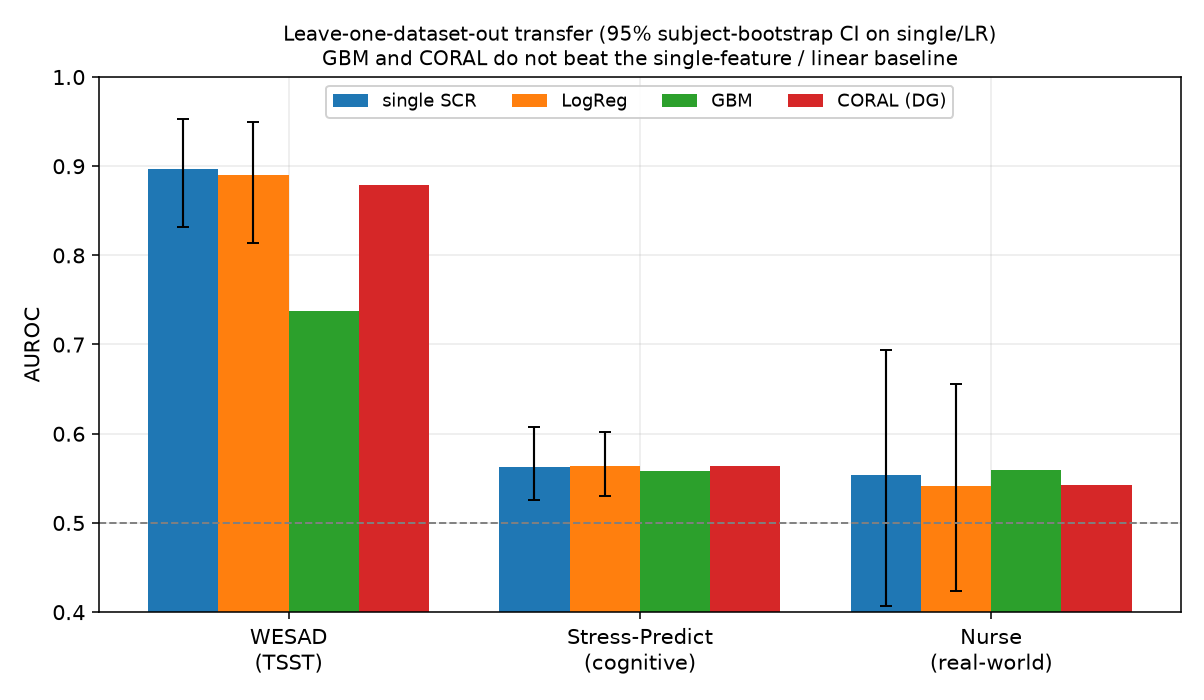
\includegraphics[width=0.92\textwidth]{figures/F1_crosscorpus.png}
\caption{Leave-one-dataset-out AUROC by model and target corpus (error bars:
95\% subject-bootstrap CI for single and logistic models). Under the evaluated
models, gradient boosting and CORAL do not exceed the
single-feature/linear baseline.\label{fig:f1}}
\end{figure}

\subsection{Four Unsupervised Adaptation Methods Do Not Recover Transfer}
\label{sec:adaptation}

Because CORAL alone cannot represent unsupervised domain adaptation, we repeated
the leave-one-dataset-out protocol with three further methods that also see the
unlabeled target distribution (Table~\ref{tab:adapt},
Figure~\ref{fig:adapt}). For subspace alignment and transfer component analysis
we report the component count that maximizes target AUROC, an optimistic upper
bound; the full grids are given in the deposited result ledger.

No method moved a weak corpus into a usable range. With Stress-Predict as target,
all six predictors fall between $0.563$ and $0.567$ and every paired difference
against the single feature contains zero. With WESAD as target, no adaptation
method meaningfully exceeded the single feature (the largest advantage was under
$0.001$ AUROC) and none was significantly worse; the weakest, transfer component
analysis, reached $0.865$ against $0.897$ with a paired difference of $+0.030$,
95\% CI $[-0.000,+0.065]$.

Nurse is the only target where an adaptation method \emph{significantly}
exceeded the single feature, that is, where the paired difference excluded zero: best-case subspace alignment reached $0.574$ against $0.553$, and
the paired difference was $-0.020$, 95\% CI $[-0.039,-0.002]$. We report this
explicitly, but it does not change the operational conclusion. The gain is
obtained by selecting the component count on target performance; across the
untuned grid the same method spans $0.538$--$0.574$. Its subject-bootstrap
interval, $[0.431,0.707]$, still includes chance, so transfer to Nurse remains
undemonstrated at the level of new subjects.

\begin{table}[H]
\centering
\caption{Leave-one-dataset-out AUROC by unsupervised adaptation method, with
95\% subject-bootstrap confidence intervals. Subspace alignment and transfer
components use the target-maximizing hyperparameters (components, and for
transfer components also the kernel bandwidth), an optimistic upper bound.
The final column is the paired subject-bootstrap difference (single SCR minus
method); an interval containing zero means the tested comparison does not
separate them. Paired differences are subject-cluster bootstrap means and need
not equal the difference of the two rounded point estimates.\label{tab:adapt}}
\begin{tabular}{llcc}
\toprule
\textbf{Target} & \textbf{Method} & \textbf{AUROC [95\% CI]} & \textbf{Single $-$ method [95\% CI]} \\
\midrule
WESAD & Single SCR (reference)   & 0.897 [0.832--0.953] & --- \\
      & Logistic, no adaptation  & 0.890 [0.814--0.949] & $+0.007$ [$-0.003$, $+0.022$] \\
      & CORAL                    & 0.879 [0.829--0.930] & $+0.018$ [$-0.007$, $+0.036$] \\
      & Subspace alignment       & 0.895 [0.818--0.954] & $+0.003$ [$-0.005$, $+0.017$] \\
      & Transfer components      & 0.865 [0.810--0.921] & $+0.030$ [$-0.000$, $+0.065$] \\
      & Importance weighting     & 0.897 [0.850--0.946] & $-0.000$ [$-0.022$, $+0.014$] \\
\midrule
Stress- & Single SCR (reference) & 0.563 [0.525--0.607] & --- \\
Predict & Logistic, no adaptation & 0.564 [0.530--0.602] & $-0.001$ [$-0.015$, $+0.015$] \\
      & CORAL                    & 0.564 [0.531--0.602] & $-0.001$ [$-0.016$, $+0.014$] \\
      & Subspace alignment       & 0.567 [0.531--0.609] & $-0.004$ [$-0.014$, $+0.007$] \\
      & Transfer components      & 0.565 [0.529--0.602] & $-0.002$ [$-0.024$, $+0.021$] \\
      & Importance weighting     & 0.565 [0.532--0.603] & $-0.002$ [$-0.020$, $+0.017$] \\
\midrule
Nurse & Single SCR (reference)   & 0.553 [0.407--0.694] & --- \\
      & Logistic, no adaptation  & 0.541 [0.423--0.656] & $+0.009$ [$-0.037$, $+0.049$] \\
      & CORAL                    & 0.542 [0.417--0.663] & $+0.009$ [$-0.016$, $+0.034$] \\
      & Subspace alignment       & 0.574 [0.431--0.707] & $-0.020$ [$-0.039$, $-0.002$] \\
      & Transfer components      & 0.571 [0.421--0.701] & $-0.017$ [$-0.063$, $+0.026$] \\
      & Importance weighting     & 0.543 [0.423--0.658] & $+0.007$ [$-0.035$, $+0.044$] \\
\bottomrule
\end{tabular}
\end{table}

\begin{figure}[H]
\centering
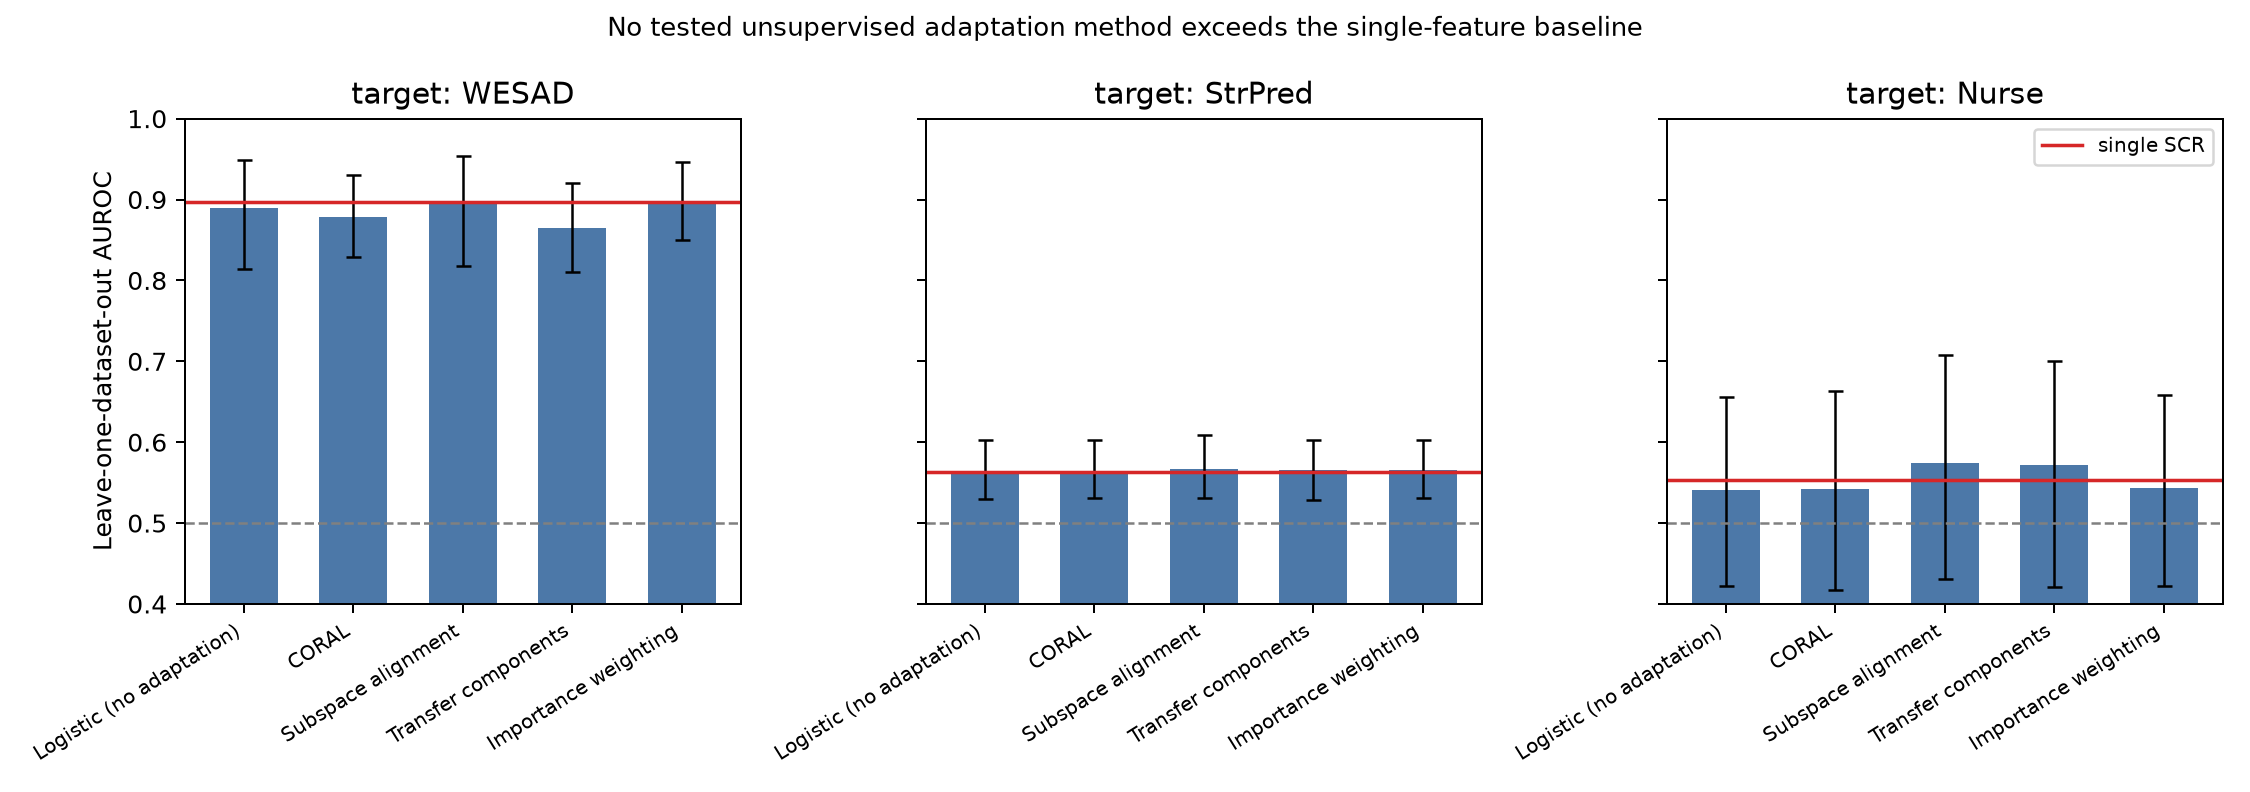
\includegraphics[width=0.98\textwidth]{figures/F8_adaptation.png}
\caption{Leave-one-dataset-out AUROC for each unsupervised adaptation method and
target corpus (error bars: 95\% subject-bootstrap CI). The red line is the
single-SCR reference and the dashed line is chance. Adaptation does not move
Stress-Predict or Nurse into a usable range.\label{fig:adapt}}
\end{figure}

Because an unsupervised method can only exploit structure the target actually
contains, we also asked what happens when target labels are supplied outright.
We trained on both source corpora plus $k$ labeled target subjects and evaluated
on the remaining subjects over 20 fixed-seed draws. Within each draw we re-scored
the source-only model on the \emph{same} held-out subjects, so the reported gain
isolates the effect of supplying labels rather than a change of evaluation
cohort. With eight labeled subjects the mean paired gain is $+0.002$ for WESAD,
$+0.001$ for Stress-Predict and $+0.029 \pm 0.024$ for Nurse. Labeling more than
half of the available Nurse participants therefore buys a small and unstable
improvement that leaves the corpus near chance, which places the limitation in
the target signal and labels rather than in the choice of adaptation method.

\subsection{Activity Context Helps Within a Corpus and Hurts Across Corpora}
\label{sec:context}

The wrist accelerometer is the one context channel available in all three
corpora, so we tested the context-aware model the translation argument implies:
the eight transfer features plus the four activity features
(Table~\ref{tab:context}, Figure~\ref{fig:context}).

Within a corpus, activity context raises every estimate. Leave-one-subject-out
AUROC rises from $0.876$ to $0.898$ (logistic) and $0.886$ to $0.930$ (boosting)
on WESAD, from $0.628$ to $0.681$ and $0.633$ to $0.671$ on Stress-Predict, and
from $0.450$ to $0.468$ (logistic) and $0.489$ to $0.572$ (boosting) on Nurse.
The Nurse logistic model nonetheless stays below chance in both variants, so the
improvement there is relative, not useful.

Across corpora the same features hurt. Leave-one-dataset-out logistic AUROC falls
from $0.890$ to $0.836$ on WESAD, $0.564$ to $0.520$ on Stress-Predict, and
$0.541$ to $0.519$ on Nurse. Boosting falls on the two weak corpora as well
($0.558$ to $0.512$ and $0.559$ to $0.545$); its WESAD value rises from $0.737$
to $0.762$ but remains far below both the single feature and plain logistic
regression. The reason is visible in the association between
movement and the stress label, which does not share a direction across corpora:
mean absolute jerk alone separates stress from non-stress at AUROC $0.828$ in
WESAD, where the speaking-and-standing protocol makes stress the more active
condition, but at $0.481$ in Stress-Predict, where the cognitive task is seated,
and $0.590$ in Nurse. A model trained on activity \emph{alone} transfers to WESAD
at $0.792$, confirming that most of what activity contributes is protocol
identity rather than stress physiology.

Activity context is therefore not a free improvement. It raises within-corpus
performance by encoding what each protocol asked participants to do, and that is
precisely the information that does not transfer to a new setting.

\begin{table}[H]
\centering
\caption{Wrist-accelerometer context-aware model. Entries are AUROC without/with
the four activity features, all else held fixed. The final column is the signed
univariate AUROC of mean absolute jerk against the stress label: above 0.5 means
more movement in stress windows, below 0.5 means less.\label{tab:context}}
\begin{tabular}{lcccc}
\toprule
& \multicolumn{2}{c}{\textbf{Within-corpus (LOSO)}} & \textbf{Transfer (LODO)} & \textbf{Movement--label} \\
\cmidrule(lr){2-3}
\textbf{Corpus} & \textbf{Logistic} & \textbf{Boosting} & \textbf{Logistic} & \textbf{AUROC (jerk)} \\
\midrule
WESAD          & 0.876/0.898 & 0.886/0.930 & 0.890/0.836 & 0.828 \\
Stress-Predict & 0.628/0.681 & 0.633/0.671 & 0.564/0.520 & 0.481 \\
Nurse          & 0.450/0.468 & 0.489/0.572 & 0.541/0.519 & 0.590 \\
\bottomrule
\end{tabular}
\end{table}

\begin{figure}[H]
\centering
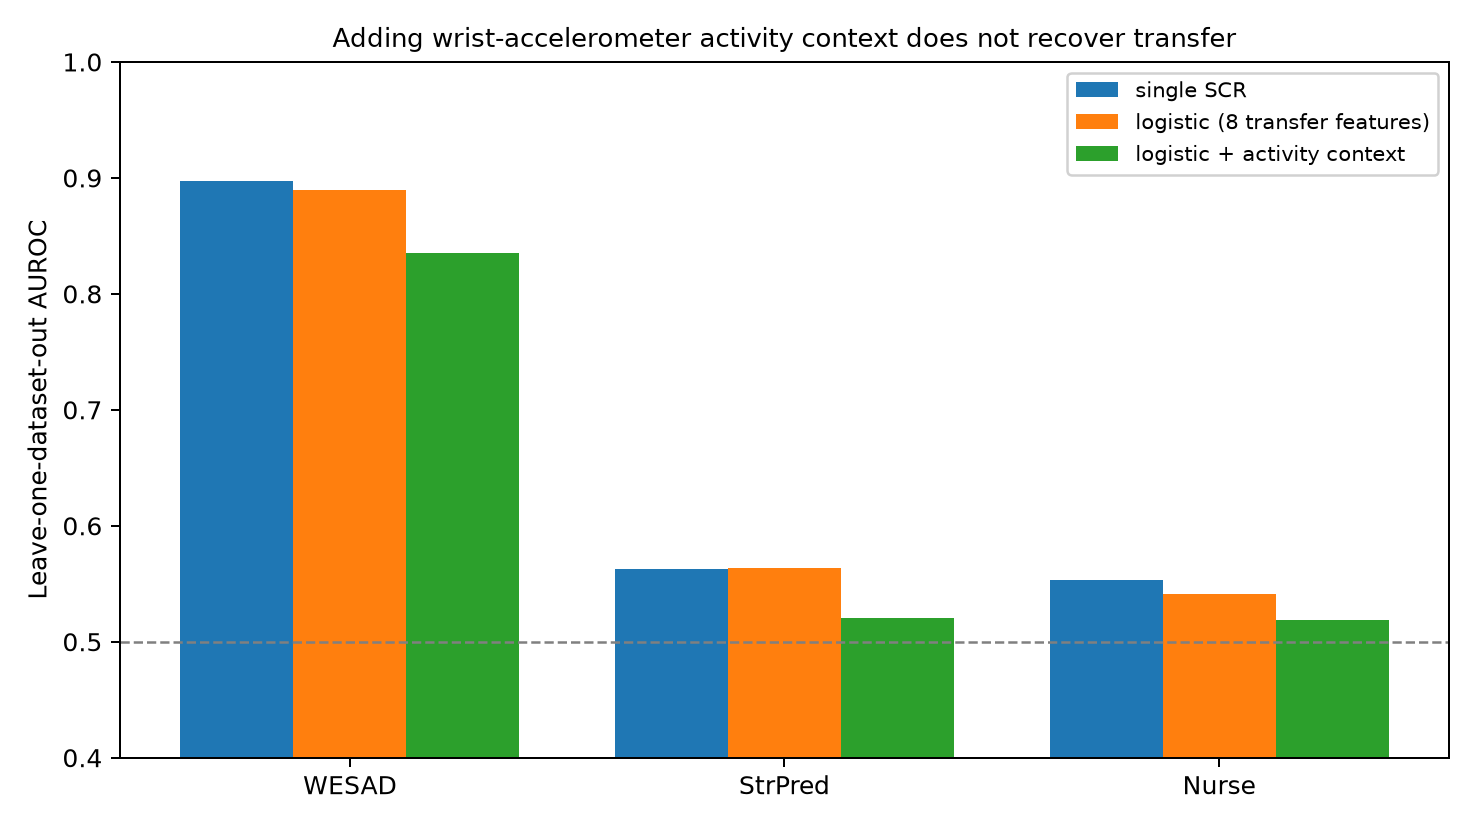
\includegraphics[width=0.72\textwidth]{figures/F9_context_aware.png}
\caption{Leave-one-dataset-out transfer with and without wrist-accelerometer
activity context. Adding activity features lowers transfer AUROC for every
target corpus, although the same features raise within-corpus
performance.\label{fig:context}}
\end{figure}

\subsection{Robustness to Windowing, HRV, and Label Alignment}

Removing window overlap leaves the leave-one-dataset-out pattern essentially
unchanged (Table~\ref{tab:window_sens}). With 300~s windows, WESAD remains the
only strong target, while Stress-Predict and Nurse remain weak. The corresponding
subject-bootstrap intervals are WESAD $0.859$--$0.974$, Stress-Predict
$0.520$--$0.611$, and Nurse $0.383$--$0.742$ for the single score; the last
interval remains especially wide because only 15 Nurse subjects are available.

\begin{table}[H]
\centering
\caption{Windowing sensitivity of leave-one-dataset-out AUROC. Each entry is
single SCR/logistic regression; all other settings are fixed.
\label{tab:window_sens}}
\begin{tabular}{lccc}
\toprule
\textbf{Window/step} & \textbf{WESAD} & \textbf{Stress-Predict} & \textbf{Nurse} \\
\midrule
64/32~s (primary) & 0.897/0.890 & 0.563/0.564 & 0.553/0.541 \\
64/64~s (non-overlap) & 0.896/0.890 & 0.564/0.563 & 0.554/0.545 \\
300/150~s & 0.917/0.913 & 0.562/0.556 & 0.564/0.522 \\
\bottomrule
\end{tabular}
\end{table}

The direct HRV ablation reaches the same conclusion
(Table~\ref{tab:hrv_sens}). Including RMSSD, SDNN, pNN50, valid-IBI count,
IBI coefficient of variation, and artifact fraction changes LOSO AUROC by at most $0.017$ at
64~s and $0.010$ at 300~s. Longer windows therefore do not reveal a previously
hidden HRV contribution that rescues the weak corpora. However, 300~s windows
reduce the available windows from 1{,}133/2{,}846/9{,}226 to
166/557/1{,}770, so the long-window estimates are sensitivity checks rather than
replacements for the primary analysis.

\begin{table}[H]
\centering
\caption{HRV-feature sensitivity for within-corpus LOSO histogram gradient
boosting. Entries are all features/the same features excluding six HRV and
quality variables. Differences quoted in the text are computed before rounding,
so they need not equal the difference of the two rounded entries.\label{tab:hrv_sens}}
\begin{tabular}{lcc}
\toprule
\textbf{Corpus} & \textbf{64~s} & \textbf{300~s} \\
\midrule
WESAD          & 0.955/0.938 & 0.959/0.965 \\
Stress-Predict & 0.675/0.672 & 0.661/0.651 \\
Nurse          & 0.621/0.616 & 0.637/0.648 \\
\bottomrule
\end{tabular}
\end{table}

Shifting every Stress-Predict protocol interval by up to one primary window in
either direction does not change the qualitative result. Across shifts from
$-64$ to $+64$~s, single-SCR AUROC ranges from $0.548$ to $0.582$ and
within-corpus logistic AUROC from $0.614$ to $0.637$ (primary alignment:
$0.563$ and $0.628$). The two series move in opposite directions
(Figure~\ref{fig:align}): the single-SCR score increases monotonically as the
protocol labels are moved later, whereas the within-corpus logistic model peaks
at $-32$~s. Alignment uncertainty can therefore contribute to the point estimate
but does not explain the weak discrimination by itself.

\begin{figure}[H]
\centering
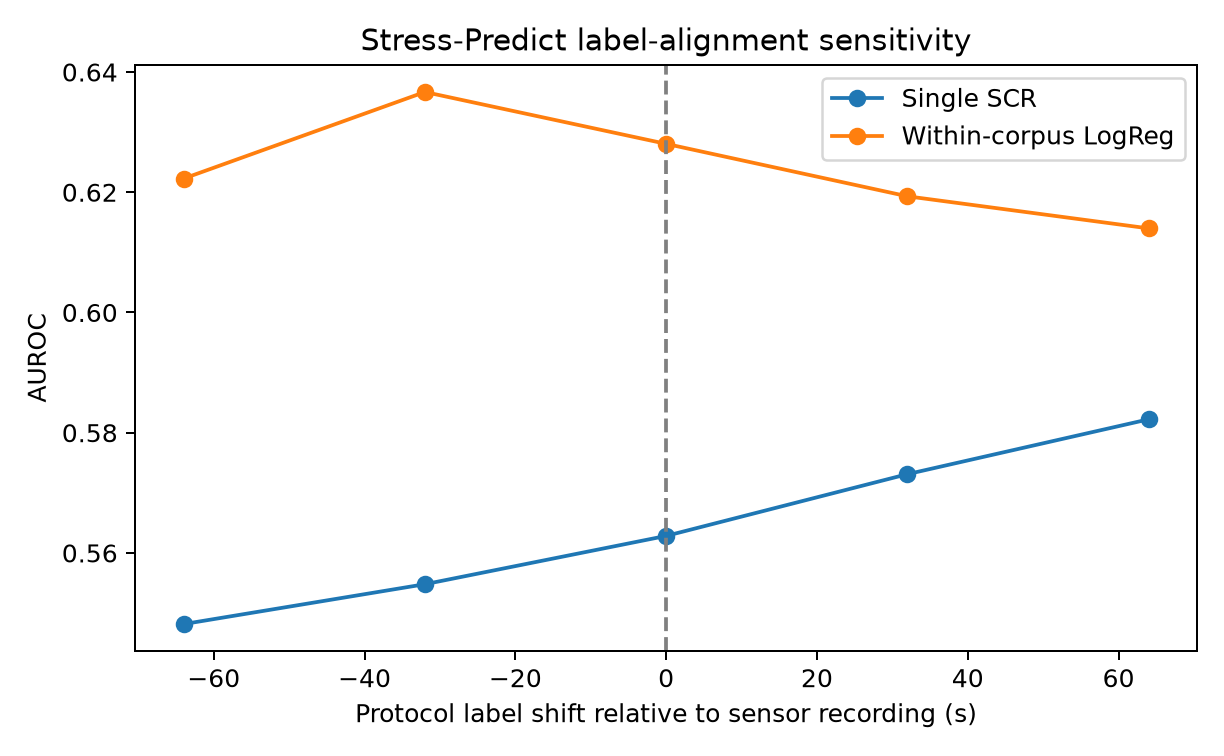
\includegraphics[width=0.66\textwidth]{figures/F6_stress_predict_alignment.png}
\caption{Stress-Predict label-alignment sensitivity. All protocol intervals are
shifted by the amount on the horizontal axis while every other analysis choice is
held fixed; the dashed line marks the primary alignment. No shift within one
window length produces strong discrimination.\label{fig:align}}
\end{figure}

Pairwise robust-standardized Wasserstein distances show measurable feature
shift (Figure~\ref{fig:f5}). Mean distance is $0.96$ for WESAD--Stress-Predict,
$1.55$ for WESAD--Nurse, and $1.61$ for Stress-Predict--Nurse; the largest
individual shifts occur in EDA decay, SCL slope, and phasic area. These
descriptive discrepancies identify candidate measurement/context differences
but cannot separate stressor type, device fit, population, and labeling quality
causally.

\begin{figure}[H]
\centering
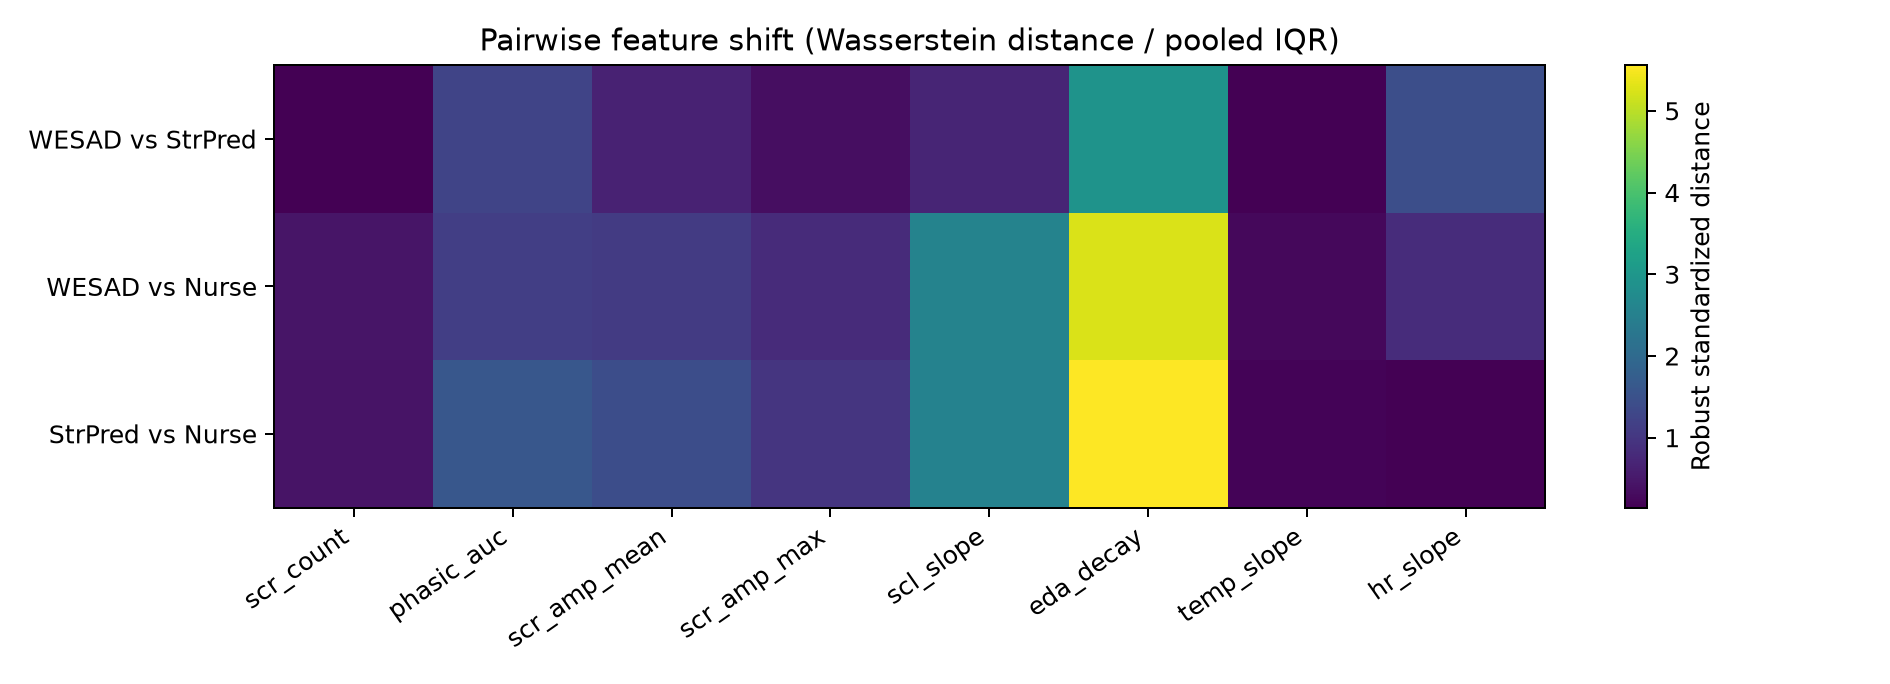
\includegraphics[width=0.92\textwidth]{figures/F5_feature_shift.png}
\caption{Pairwise distribution shift for the eight transfer features. Each cell
is a one-dimensional Wasserstein distance divided by the pairwise pooled
interquartile range; larger values indicate greater marginal discrepancy, not a
causal contribution to error.\label{fig:f5}}
\end{figure}

\subsection{Iso-HR Evidence Is Diagnostic Mainly in WESAD}
\label{sec:isohr}

The iso-HR decomposition (Table~\ref{tab:isohr}, Figure~\ref{fig:f3}) gives an
HR-leakage index of $\approx$0 in every corpus (WESAD $+0.020\pm0.008$,
Stress-Predict $-0.001\pm0.006$, Nurse $-0.006\pm0.006$ over seven matching
seeds): HR \emph{level} adds essentially nothing once the other signals are
present. As cautioned in the Methods, a near-zero index is informative only where
a signal exists. The decisive case is WESAD, where matching HR barely changes
performance (all-feature AUROC $0.955\rightarrow0.938\pm0.009$) \emph{and} the
purely non-cardiac (EDA+temperature) signal remains strong after matching
($0.935\pm0.015$); this argues against an HR confound as the explanation for
WESAD's signal. For Stress-Predict and Nurse the matched non-cardiac AUROC is near
chance ($0.607\pm0.016$ and $0.548\pm0.007$), so the near-zero leakage there is a
floor effect: nothing discriminates, including HR. Taken together, the
WESAD result argues against HR-level confounding as the main explanation for its
signal. The weak Stress-Predict and Nurse signals do not distinguish among label
noise, device fit, stressor type, population, and workflow context. The small
standard deviations across seeds confirm that this bounded decomposition is not
a single-draw artifact.

\begin{table}[H]
\centering
\caption{Per-corpus iso-HR decomposition (AUROC). ``Unmatched (all)'' is
deterministic; matched columns are mean\,$\pm$\,standard deviation (SD) over
seven matching seeds (the
matched subsample is random). ``Non-cardiac'' is EDA\,+\,temperature only. The
HR-leakage index $=$ matched(all) $-$ matched(HR-level-free), where
``HR-level-free'' excludes mean HR and mean IBI but still retains cardiac
dynamics and HRV; it is near zero everywhere, while the matched non-cardiac signal
is strong only for social-evaluative stress.\label{tab:isohr}}
\begin{tabular}{lcccr}
\toprule
\textbf{Corpus} & \textbf{Unmatched} & \textbf{Matched} & \textbf{Matched} & \textbf{HR-leakage} \\
 & \textbf{(all)} & \textbf{(all)} & \textbf{(non-cardiac)} & \textbf{index} \\
\midrule
WESAD          & 0.955 & $0.938\pm0.009$ & {\boldmath$0.935\pm0.015$} & $+0.020\pm0.008$ \\
Stress-Predict & 0.675 & $0.640\pm0.017$ & $0.607\pm0.016$ & $-0.001\pm0.006$ \\
Nurse          & 0.621 & $0.544\pm0.008$ & $0.548\pm0.007$ & $-0.006\pm0.006$ \\
\bottomrule
\end{tabular}\\[2pt]
{\footnotesize Matched windows $n$: WESAD 318, Stress-Predict 1{,}524, Nurse 2{,}210.}
\end{table}

\begin{figure}[H]
\centering
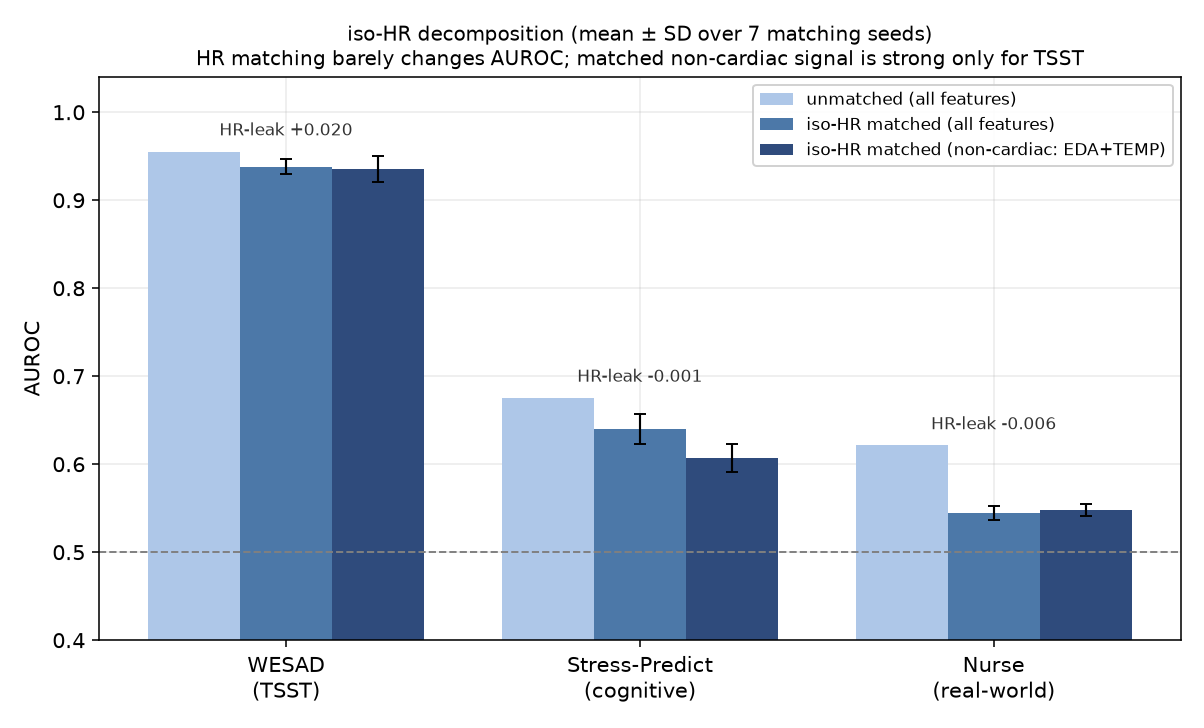
\includegraphics[width=0.85\textwidth]{figures/F3_isohr_decomp.png}
\caption{Iso-HR decomposition (bars: unmatched all-feature, iso-HR matched
all-feature, and iso-HR matched non-cardiac [EDA+temperature]; error bars are SD
over seven matching seeds). Heart-rate matching barely changes AUROC (HR-leakage
$\approx$0), and the matched non-cardiac signal is strong only for laboratory
social-evaluative stress (WESAD). The two weak-signal corpora remain
floor-effect-limited and do not support causal attribution.\label{fig:f3}}
\end{figure}

\subsection{The Nurse Evaluation Shows Weak Operational Discrimination}

Stratifying Nurse windows into movement tertiles leaves AUROC near chance
throughout (Figure~\ref{fig:f2}: single-feature
$0.476$/$0.566$/$0.504$ for low/mid/high movement; logistic below $0.5$).
The absence of a monotonic movement effect means motion alone does not account
for the pattern, but it does not identify whether weak physiology, device fit,
context, or retrospective labels dominate.

\begin{figure}[H]
\centering
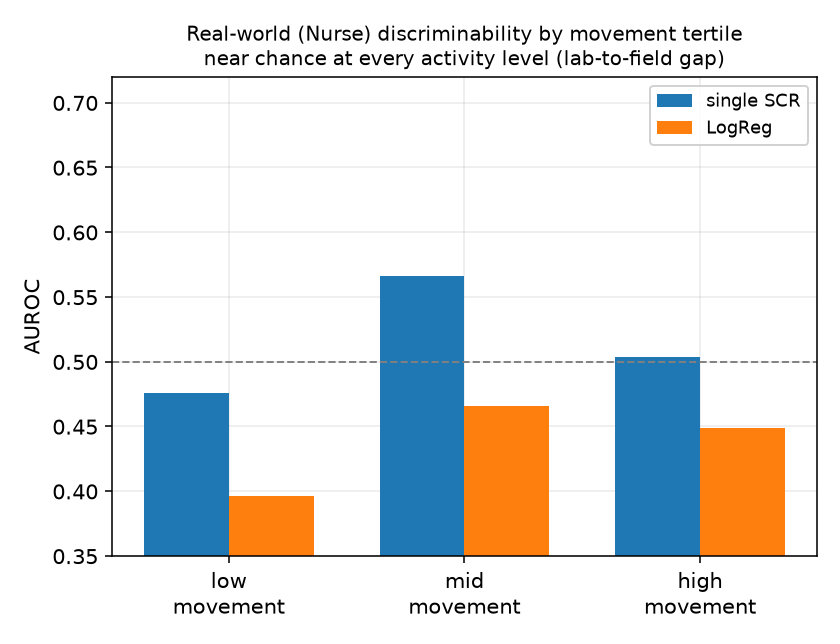
\includegraphics[width=0.6\textwidth]{figures/F2_nurse_movement.png}
\caption{Real-world (Nurse) discriminability by movement tertile. AUROC remains
near chance at all activity levels; movement stratification does not resolve the
source of weak discrimination.\label{fig:f2}}
\end{figure}

The operational metrics reinforce this uncertainty (Table~\ref{tab:nurse_util},
Figure~\ref{fig:f4}). Average precision of $0.826$--$0.828$ is only
$0.030$--$0.032$ above the stress prevalence of $0.796$. At the fixed 0.5
threshold, logistic regression detects $58.3\%$ of stress windows but falsely
flags $53.5\%$ of non-stress windows; gradient boosting lowers the false-positive
rate to $27.5\%$ while detecting only $35.6\%$ of stress windows. Calibration is
also poor (ECE $0.238$ and $0.378$). These values do not support an operational
alerting system under the present labels. Because the labels are sparse,
retrospective, and imbalanced, they also do not establish that the underlying
physiology cannot transfer.

\begin{table}[H]
\centering
\caption{Nurse leave-one-dataset-out operational metrics. Logistic regression
and gradient boosting are trained on WESAD and Stress-Predict; threshold 0.5 is
fixed without Nurse-label tuning. ECE is 10-bin expected calibration error.
\label{tab:nurse_util}}
\begin{tabular}{lrrrrrrr}
\toprule
\textbf{Model} & \textbf{AUROC} & \textbf{AP} & \textbf{Brier} &
\textbf{ECE} & \textbf{Bal.\ acc.} & \textbf{Sens.} & \textbf{FPR} \\
\midrule
Single SCR & 0.553 & 0.826 & -- & -- & -- & -- & -- \\
Logistic   & 0.541 & 0.826 & 0.243 & 0.238 & 0.524 & 0.583 & 0.535 \\
Boosting   & 0.559 & 0.828 & 0.344 & 0.378 & 0.541 & 0.356 & 0.275 \\
\bottomrule
\end{tabular}
\end{table}

\begin{figure}[H]
\centering
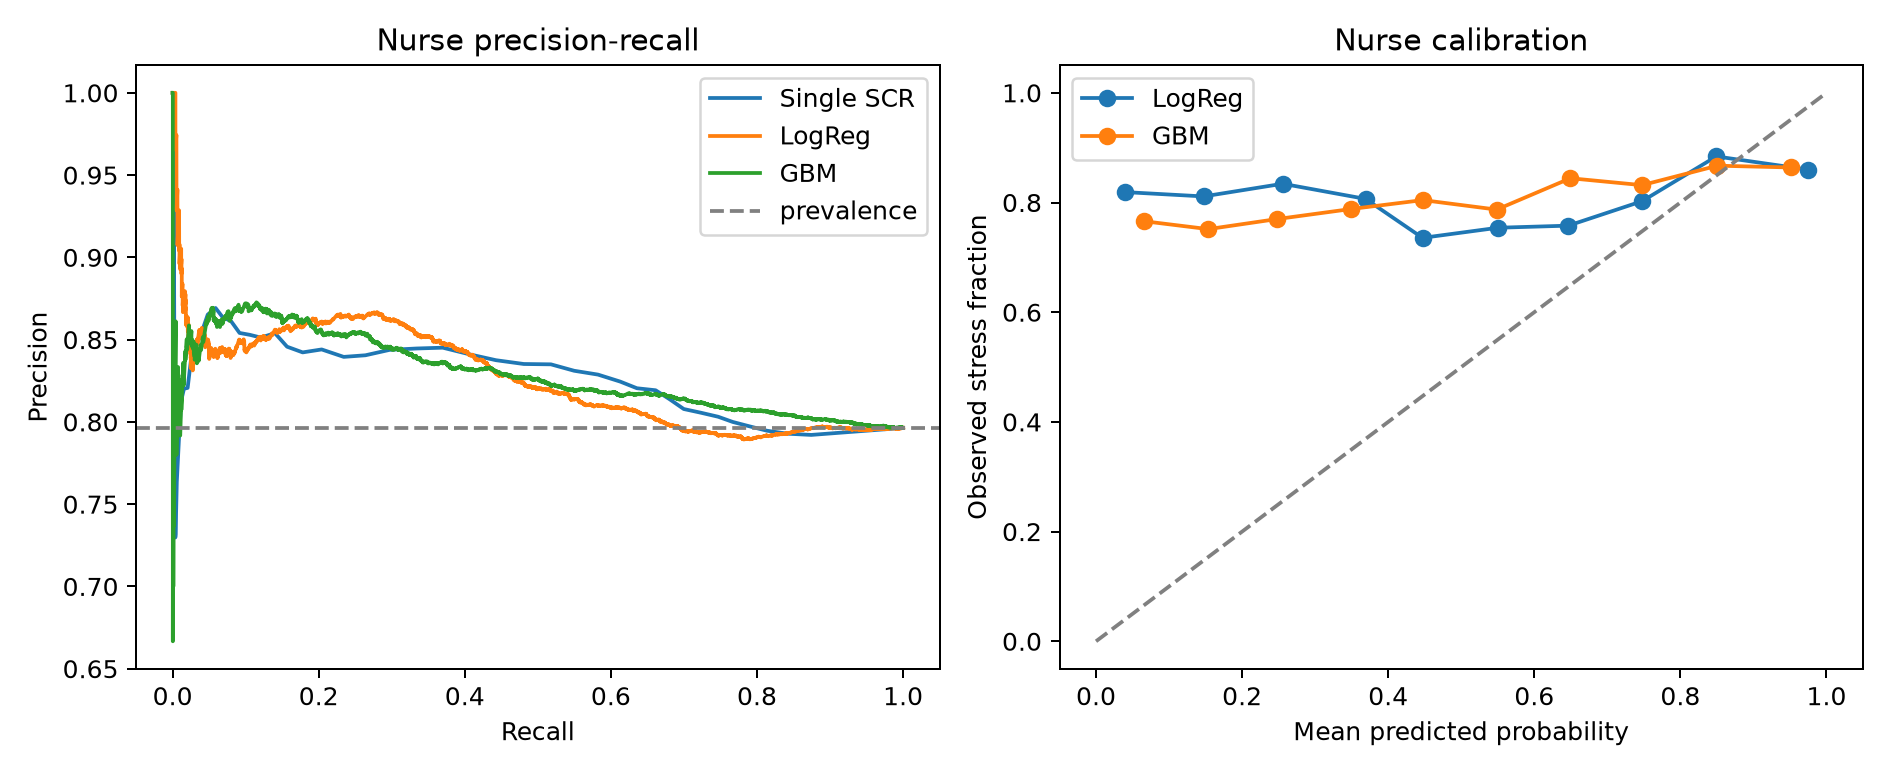
\includegraphics[width=0.92\textwidth]{figures/F4_nurse_utility.png}
\caption{Nurse precision--recall curves (left) and reliability curves for the
probabilistic source-trained models (right). The dashed precision baseline is
the target prevalence ($0.796$); the diagonal is perfect calibration.
\label{fig:f4}}
\end{figure}

% =====================================================================
\subsection{Error Stratification Locates the Residual Nurse Discrimination}
\label{sec:errstrata}

To describe where transfer errors concentrate, we stratified the fixed
source-trained scores---without refitting---by movement level, HR band, beat
quality, and Mahalanobis distance to the source feature distribution, and
combined the within-stratum AUROCs with $n_{\text{stress}} \times
n_{\text{non-stress}}$ weights (Table~\ref{tab:errstrata},
Figure~\ref{fig:errstrata}). The quantity of interest is the gap between the
pooled and the within-stratum estimate: the part of apparent discrimination that
comes from score offsets \emph{between} strata rather than ranking \emph{inside}
them.

For Nurse, that gap consumes the entire effect. Pooled logistic AUROC is $0.541$,
but conditioning on distance to the source distribution leaves $0.489$, and
conditioning on movement tertile leaves $0.499$---at or below chance in both
cases. The already weak Nurse signal is therefore largely a between-context
offset rather than within-context ranking. The per-subject picture agrees:
of 15 Nurse subjects, 13 have both classes, and their logistic AUROC has median
$0.511$ and range $0.370$--$0.725$, so roughly half fall below chance.

WESAD behaves differently: conditioning reduces AUROC from $0.890$ to $0.826$
(distance) and $0.857$ (movement) but leaves it clearly above chance, and 15 of
15 subjects are evaluable with median $0.985$. One WESAD stratum is a useful
caution, however: in the 102 windows at or above the $0.0796$~g movement gate,
discrimination collapses to $0.530$ (single) and $0.467$ (logistic), so even the
strongest corpus loses its signal once participants are physically active.

Stress-Predict shows no comparable concentration; every stratified estimate stays
within $0.036$ of the pooled value.

These strata are observed conditions, not manipulated factors, so a difference
between strata is an association and does not by itself identify a cause.

\begin{table}[H]
\centering
\caption{Leave-one-dataset-out error stratification for the logistic model.
``Within-stratum'' combines stratum-specific AUROCs with
$n_{\text{stress}} \times n_{\text{non-stress}}$ weights; ``between-stratum
share'' is pooled minus within-stratum. A large positive share means the pooled
value is carried by score offsets between strata rather than by ranking inside
them.\label{tab:errstrata}}
\begin{tabular}{llccc}
\toprule
\textbf{Target} & \textbf{Stratifier} & \textbf{Pooled} & \textbf{Within-stratum} & \textbf{Between-stratum share} \\
\midrule
WESAD & Movement tertile        & 0.890 & 0.857 & $+0.033$ \\
      & Movement gate (0.0796~g) & 0.890 & 0.895 & $-0.005$ \\
      & HR band                 & 0.890 & 0.912 & $-0.023$ \\
      & Beat quality            & 0.890 & 0.851 & $+0.038$ \\
      & Distance to source      & 0.890 & 0.826 & $+0.064$ \\
\midrule
Stress- & Movement tertile      & 0.564 & 0.600 & $-0.036$ \\
Predict & Movement gate         & 0.564 & 0.574 & $-0.011$ \\
      & HR band                 & 0.564 & 0.549 & $+0.015$ \\
      & Beat quality            & 0.564 & 0.561 & $+0.003$ \\
      & Distance to source      & 0.564 & 0.557 & $+0.007$ \\
\midrule
Nurse & Movement tertile        & 0.541 & 0.499 & $+0.042$ \\
      & Movement gate           & 0.541 & 0.506 & $+0.036$ \\
      & HR band                 & 0.541 & 0.559 & $-0.018$ \\
      & Beat quality            & 0.541 & 0.559 & $-0.018$ \\
      & Distance to source      & 0.541 & 0.489 & $+0.052$ \\
\bottomrule
\end{tabular}
\end{table}

\begin{figure}[H]
\centering
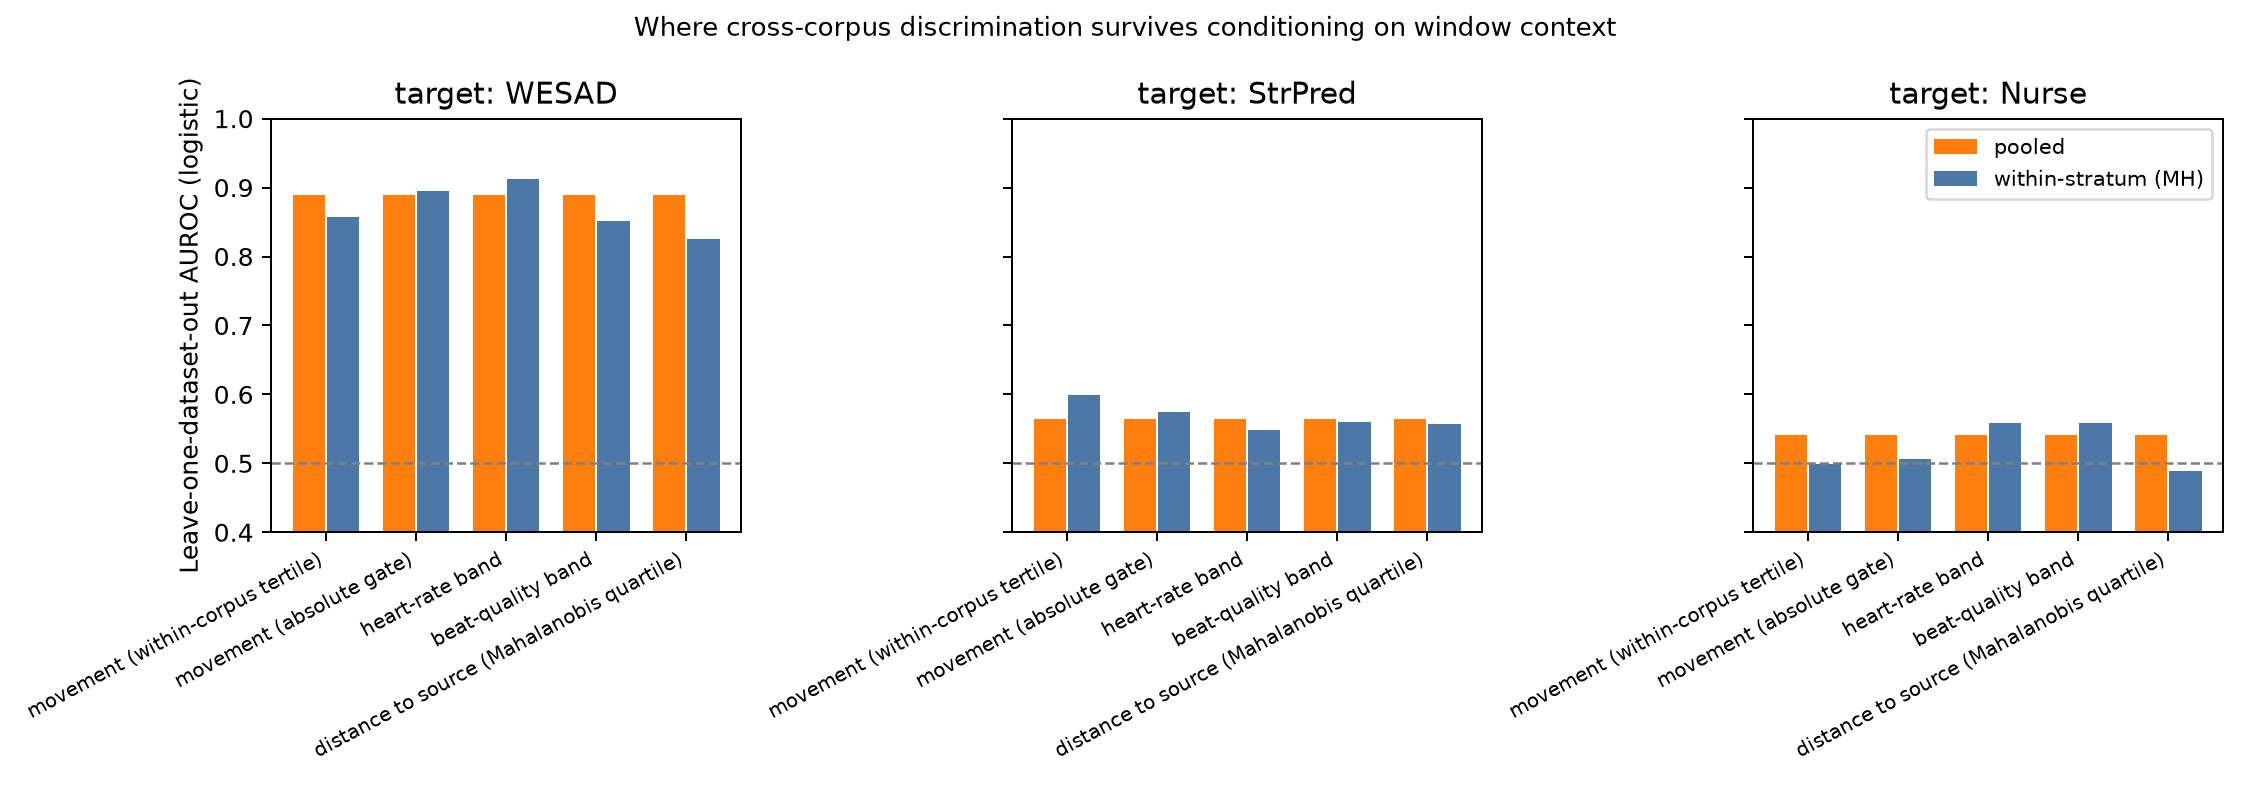
\includegraphics[width=0.98\textwidth]{figures/F10_error_strata.png}
\caption{Pooled versus within-stratum leave-one-dataset-out AUROC for the
logistic model. For Nurse, conditioning on movement level or on distance to the
source distribution removes the residual discrimination
entirely.\label{fig:errstrata}}
\end{figure}

% =====================================================================
\section{Discussion}
% =====================================================================

This study reframes wearable stress detection as a clinical-informatics
translation problem. The key result is not simply that one model outperformed
another. Rather, the same physiological measurements that appear useful in a
controlled stress protocol become weak and unstable when moved into a physically
active nursing workflow. For Healthcare applications, this distinction is
critical: a stress score deployed in a ward would not be consumed as an abstract
AUROC value, but as a possible alert, dashboard signal, or workforce-management
input. If such a signal is not transferable, it can add interruption and
operational noise instead of helping clinicians. In the language of digital
medicine validation, the present findings are an analytical and translational
warning: a wearable-derived measure may be technically computable and
within-dataset predictive, yet still not be fit for a new clinical context of
use~\cite{goldsack2020v3,manta2020digitalmeasures}.

Four findings define the boundary. First, added model complexity did not solve
the translation problem. A single SCR feature matched or exceeded logistic
regression, histogram boosting and four unsupervised adaptation methods where the
signal was strong, and none of them produced reliable Nurse discrimination. The
one exception is instructive rather than encouraging: best-case subspace
alignment beat the single feature on Nurse by $0.020$ AUROC, but only after its
component count was chosen on target performance, and its subject-bootstrap
interval still spans chance. Adversarial representation learning remains untested,
and supplying target labels directly did not stabilize Nurse either; what the
present evidence shows is that complexity alone is not evidence of transfer when
the target labels and signal are weak.

This finding aligns with the broader literature on wearable stress monitoring,
which increasingly recognizes that model generalization, labeling quality, and
context are central limitations rather than minor implementation
details~\cite{vos2023generalizable,tutunji2023prolonged}. Studies in office-like
environments and cross-context prediction frameworks show that behavioral and
contextual signals may carry information that physiological channels alone do not
capture~\cite{naegelin2023interpretable,mihirette2025crosscontextual}. Our
results extend that logic to nursing work: the absence of reliable Nurse-corpus
discrimination should not be read as a failure of EDA as a signal in general.
Under sparse retrospective labels it is equally compatible with weak physiology,
label mismatch, device fit, and an under-specified workflow model.

Second, iso-HR matching shows that the result cannot be reduced to a simple
heart-rate-confounding story. In WESAD, where a strong signal exists, the
non-cardiac EDA+temperature signal remains strong after HR matching. This supports
the physiological plausibility of EDA-based stress detection under a
social-evaluative laboratory stressor. In Stress-Predict and Nurse, however, all
matched feature sets remain weak. The near-zero HR-leakage index in these corpora
is therefore a floor effect rather than proof of robust stress specificity. The
interpretation is clinically important: the problem is not only that HR shortcuts
can mislead models, but also that the two weak corpora do not provide enough
discrimination to identify a single explanation for transfer failure.

This point also sharpens the role of physical activity. Recent acute
stress-versus-exercise data demonstrate that stress and exercise can be measured
with overlapping wrist channels while still requiring explicit contextual
separation~\cite{hongn2025wearable}. Our iso-HR result is consistent with that
view. HR matching is necessary but not sufficient: it removes the most direct
cardiac shortcut, yet it cannot fully resolve ambiguity introduced by movement,
task demands, thermal context, and retrospective labeling in a real clinical
shift.

Third, the Nurse corpus should be treated as an ecologically demanding
context-of-use test rather than as a failed benchmark or a nurse-specific
prediction target. Its physiological recordings are embedded in patient care,
movement, interruptions, and delayed self-report. In the original Nurse dataset,
ecological momentary assessments were collected at sparse intervals, which means
that minute-by-minute physiological triggers are not directly
annotated~\cite{hosseini2022nurse}. A label describing high stress across a
multi-hour period may mix acute psychological strain, physical workload, baseline
fatigue, and contextual pressure. Under this labeling structure, a wearable model
may be asked to solve a problem that the available ground truth cannot cleanly
define. This does not make the Nurse result proof of physiological non-transfer;
it makes the corpus a realistic test of both measurement and ground-truth
limitations in field-based clinical informatics.

This interpretation follows from the operational definition in
Table~\ref{tab:contextdefinition}. The three corpora are deliberately used as
different context-of-use probes rather than as exchangeable sources of more
training data. WESAD asks whether a clear physiological stress signal is
detectable under controlled conditions; Stress-Predict asks whether that signal
survives a milder cognitive-stressor shift; Nurse asks whether the same class of
wearable output remains meaningful when embedded in clinical work. Under this
definition, low Nurse-corpus transfer is not a secondary inconvenience. It is a
healthcare validity warning, but the wide subject interval and label limitations
prevent a definitive physiological conclusion. A model that works in
wellness-like conditions but remains weak in this boundary case should not be
interpreted as ready for healthcare workforce dashboards or alerts.

Fourth, the bounded robustness analyses do not reveal a simple technical repair.
Non-overlapping and 300~s windows preserve the transfer pattern, six HRV/quality
features change AUROC by at most 0.017, plausible Stress-Predict label shifts do
not create strong discrimination, and four unsupervised adaptation methods leave
the weak corpora weak. Error stratification adds the one positive localization we
can make: for Nurse, conditioning on movement level or on distance to the source
distribution removes the residual discrimination entirely
(Section~\ref{sec:errstrata}), so what little the pooled estimate contains is a
between-context offset rather than within-context ranking. The marginal feature
shifts and the strata remain descriptive rather than causal, but together they
point away from a missing-model explanation and toward context and label quality.

\subsection{Interpreting Negative Transfer as Healthcare Evidence}

Negative transfer is often treated as an engineering problem: the model did not
generalize, so the next step is to add more features, more data, or a stronger
domain-adaptation method. We took two of those steps. Three additional
unsupervised adaptation methods (Section~\ref{sec:adaptation}) and an
accelerometer context-aware model (Section~\ref{sec:context}) left the weak
corpora weak, and the context features actively reduced transfer because they
encode protocol rather than physiology. That interpretation is therefore partly
correct, but incomplete for healthcare. In a context-of-use framework, failure to transfer is itself a
form of evidence. It identifies the boundary at which a digital measure no
longer represents the construct that users may believe it
represents~\cite{goldsack2020v3,manta2020digitalmeasures}. For a consumer
wellness score, this boundary may be acceptable if the output is used only for
personal reflection. For a healthcare workforce signal, the same boundary has
practical meaning because the output may be interpreted as a marker of work
strain, risk, or need for intervention.

This distinction is important for the present findings. The Nurse corpus does
not merely lower the average cross-corpus AUROC. It changes the interpretation of
the entire pipeline. A model that performs well on WESAD but fails under
naturalistic nursing work is not simply a model with poor external validation; it
is a model whose apparent construct validity is conditional on a narrow stressor
and activity context. The high WESAD result shows that wrist EDA can carry a
detectable stress signal under a strong, well-defined social-evaluative protocol.
The weak Nurse result shows that this signal does not automatically remain a
healthcare-workflow measure. Both results are necessary for the translational
claim. Without the positive benchmark result, there would be little physiological
signal to translate. Without the negative healthcare boundary result, the
benchmark could be overread as deployment evidence.

This also affects how future model improvements should be judged. A more complex
classifier, additional sensor channels, or domain adaptation may improve
cross-corpus performance, but such improvement would not by itself establish
clinical utility~\cite{vickers2006decisioncurve,vancalster2019calibration}. The
improved model would still need to show what construct it measures in the
clinical workflow, whether its errors cluster around predictable tasks, and
whether its output changes a decision in a beneficial way.
Conversely, a simple model may be preferable if it has a narrower but more
transparent use, for example identifying intervals of physiological arousal for
later voluntary reflection rather than generating real-time alerts. The
methodological lesson is therefore not that public nurse datasets are too noisy
to be useful. It is that their noise, sparsity, and workflow complexity are
precisely what reveal the gap between benchmark validity and healthcare
validity.

These findings connect directly to patient-safety and human-factors concerns.
Healthcare already struggles with alert burden, repeated alerts, cognitive load,
and alarm fatigue~\cite{ancker2017alertfatigue,lewandowska2020alarmfatigue,
ruppel2023alarmburden,gulsen2025alarmfatigue}. A consumer smartwatch stress
score or wellness dashboard signal that mistakes physical work for psychological
strain could become another low-specificity notification stream. This concern is
not hypothetical in healthcare workforce contexts, where workload, burnout,
staffing, and alarm burden are already linked to staff well-being, perceived
safety, care quality, and patient
safety~\cite{dallora2020burnout,hall2016staffwellbeing,ruppel2023alarmburden,
gulsen2025alarmfatigue}.
Even if such a system is framed as staff wellness rather than patient monitoring,
its outputs could influence attention, self-perception, staffing dashboards, or
occupational health decisions. The appropriate standard is therefore higher than
within-dataset classification accuracy. A wearable stress metric intended for
healthcare workflows should demonstrate transfer across stressor types,
robustness under HR control, and acceptable false-positive behavior at realistic
field prevalence.

\subsection{Clinical and Informatics Implications}

The clinical utility question is therefore narrower, and more demanding, than the
usual benchmark question. A wrist-derived stress score is not a diagnosis, a
validated workload measure, or an immediately actionable alert by itself. Its
value depends on whether the score improves a specified healthcare decision
without adding cognitive, operational, or interpretive burden. In a private
wellness setting, a noisy stress estimate may be tolerable because the user can
ignore it. In a healthcare workforce setting, the same signal may be routed into
dashboards, staffing discussions, occupational-health interpretations, or
well-being interventions. The relevant evidence standard is therefore not only
``Can the model distinguish labeled stress windows?'' but ``Does the measure
remain meaningful, specific, and useful in the intended clinical
workflow?''~\cite{goldsack2020v3,manta2020digitalmeasures,vickers2006decisioncurve}.

The single-SCR result has a direct design implication. If a fixed,
physiologically interpretable feature performs on par with logistic regression or
gradient boosting where a stress signal exists, then added model complexity
requires its own justification. For healthcare workforce applications, a simpler
feature can reduce computation, ease on-device or edge deployment, and make the
output easier to audit~\cite{naegelin2023interpretable}. It also gives
clinicians, occupational-health teams, and system designers a clearer account of
what the device is reacting to: discrete skin-conductance responses rather than
an opaque weighted combination of many features. This does not mean that
multivariate models are unnecessary in all future systems, but it does mean that
complexity should be added only when it improves transfer, calibration,
false-alert behavior, or decision value beyond an interpretable physiological
baseline.

This is a shift from benchmark validity to healthcare context-of-use validity,
as set out by digital-measure validation frameworks~\cite{goldsack2020v3,
manta2020digitalmeasures,vancalster2019calibration,vickers2006decisioncurve} and
summarized against the corresponding validation requirements in
Table~\ref{tab:validationmap}. The criteria also clarify why the Nurse corpus is
informative even when AUROC is low. Poor transfer in this setting indicates that
the measure cannot yet support clinical workforce interpretation without
additional context, not simply that one dataset is difficult.

\subsection{Deployment Failure Modes and Prospective Validation Needs}

The practical implication is not that wrist wearables have no role in healthcare
workforce monitoring. Instead, they should be embedded in context-aware
informatics designs that explicitly anticipate deployment failure
modes~\cite{virgillito2025wearablesorg}. The first failure mode is a
false-positive workflow signal. A wrist model may flag patient transfer, rapid
walking to a call light, donning or doffing equipment, or heat exposure as
stress. In a private wellness application, such a signal may be annoying but
inconsequential. In a clinical workforce setting, repeated false-positive scores
could become another low-specificity notification stream, contribute to alert
burden, or create avoidable concern about normal clinical
activity~\cite{ancker2017alertfatigue,lewandowska2020alarmfatigue,
ruppel2023alarmburden,gulsen2025alarmfatigue}. The second failure mode is a
false-negative emotional signal. A clinician may experience distress during a
difficult conversation,
conflict, error recovery, or end-of-life care without producing the same
physiological pattern as a laboratory stressor. A model that misses such events
could provide misleading reassurance if the score is interpreted as a workload or
well-being indicator.

A third failure mode is aggregation error. Stress scores are often easier to
display at the shift, unit, or staff-group level than to interpret at the
minute-by-minute level. However, aggregating noisy physiological estimates can
make them appear more stable and objective than the underlying labels justify.
This is especially important for healthcare workforce monitoring because the
same dashboard value could be read as a personal wellness trend, an occupational
health concern, a staffing signal, or a proxy for care pressure. The fourth
failure mode is governance drift: a signal introduced for individual reflection
may gradually become part of performance management, staffing review, or
organizational surveillance. Even when no patient data are involved, workforce
stress monitoring is not ethically neutral because it measures clinicians during
work and may be interpreted by people other than the
wearer~\cite{martinezmartin2021ethical,ajunwa2017surveillance}. These risks make
the ``intended use'' of the measure a methodological variable, not only a
deployment detail.

Future systems may therefore need to combine physiology with passive context such
as activity state, shift timing, task category, location within the care
environment, or workload metadata. Rather than one monolithic stress model,
clinical systems may require modular submodels that interpret physiological
deviations within the operational context in which they occur. Such designs would
better align with the realities of nursing work, where the same HR or EDA pattern
may mean patient transfer, urgent response, heat exposure, anxiety, or emotional
distress depending on context. Table~\ref{tab:validationmap} translates this
argument into validation requirements for future Healthcare-oriented wearable
stress studies, alongside the benchmark framing each requirement replaces.

\begin{table}[H]
\centering
\caption{From benchmark validity to healthcare context-of-use validity: the
requirement, rationale, and example design for each validation dimension before
healthcare workforce deployment.\label{tab:validationmap}}
\begin{tabular}{@{}L{0.12\textwidth}L{0.17\textwidth}L{0.26\textwidth}L{0.19\textwidth}L{0.19\textwidth}@{}}
\toprule
\textbf{Validation dimension} & \textbf{Benchmark framing} & \textbf{Healthcare
context-of-use requirement} & \textbf{Healthcare rationale} & \textbf{Example
study design} \\
\midrule
Construct validity &
Classify stress labels within a known corpus. &
Determine whether the wearable signal represents a clinically interpretable state
under physical work, interruptions, alarms, and delayed self-report; prespecify
whether the target is acute stress, workload, fatigue, distress, or a broader
well-being state. &
Different constructs imply different actions and different risks of
misinterpretation. &
Combine time-stamped self-report with event-level clinical annotations. \\
Activity robustness and transfer &
Use subject-disjoint cross-validation within one dataset. &
Demonstrate transfer across stressor types, HR distributions, activity contexts,
and field labeling conditions, and show that performance survives HR control,
movement context, posture, and shift-related physical work. &
Physical care tasks can resemble stress physiology at the wrist. &
Evaluate models within matched activity strata and report false positives during
patient-care tasks. \\
Workflow specificity &
Report a model that performs well on public data. &
Prespecify the intended use, users, action pathway, and false-alert tolerance:
where the score appears, who sees it, and what action it supports. &
A score used for private reflection has a different burden than a staffing or
occupational-health signal. &
Prospectively test a dashboard or alert pathway with prespecified users and
actions. \\
Incremental decision value &
Maximize discrimination metrics such as AUROC. &
Show that the measure supports a specified workflow, occupational-health, or
well-being decision beyond contextual baselines such as shift type, workload,
task category, or alarm exposure. &
A wearable measure should add decision value beyond information already available
in the work system. &
Report whether wearable features improve calibration, discrimination, or
decision curves over contextual models. \\
False-alert burden &
Misclassification lowers model performance. &
Quantify alert frequency, false-positive clusters, and user response under field
prevalence, recognizing that ambiguous scores add alert burden, staff concern,
and dashboard noise. &
Even accurate models can fail if they create interruption or dashboard noise. &
Use prospective monitoring with alert-suppression rules and workload-sensitive
thresholds. \\
Governance and privacy &
Not addressed in benchmark reporting. &
Specify data access, retention, aggregation, consent, and non-punitive use. &
Workforce monitoring can affect trust even when framed as wellness support. &
Evaluate acceptability with clinicians, managers, and occupational-health
stakeholders before deployment. \\
\bottomrule
\end{tabular}
\end{table}

These requirements also imply a different reporting standard from conventional
classification papers. AUROC remains useful for separating models, but it is
insufficient for deciding whether a stress score should appear in a clinical
workflow. A healthcare-facing evaluation should report calibration, expected
false-positive counts per shift, positive predictive value under field
prevalence, and performance within clinically relevant activity
states~\cite{vancalster2019calibration,vickers2006decisioncurve}. A model with
acceptable AUROC can still be unusable if it fires repeatedly during normal
rounding, patient transfers, or alarm response. Conversely, a modest classifier
may be useful if it is restricted to a narrow action pathway, such as prompting
optional self-reflection after a high-burden interval, and if it remains silent
during predictable physical work.

Threshold selection is therefore part of clinical design rather than a purely
statistical afterthought. In wellness applications, a threshold can be tuned for
user engagement or subjective plausibility. In healthcare workforce settings,
the same threshold defines who is interrupted, what is shown to supervisors or
occupational-health teams, and how often normal care activity is reframed as
stress. Future studies should therefore prespecify whether outputs are
individual-only, aggregated for unit-level monitoring, or connected to an action
by another party. Without that specification, model performance cannot be
translated into clinical utility because the cost of an error is
undefined~\cite{vickers2006decisioncurve,martinezmartin2021ethical}.

This framing also changes what a successful next study should look like. Rather
than optimizing a single model on one corpus, future Healthcare-oriented wearable
stress studies should prespecify the intended decision context, collect
time-resolved labels close to clinically meaningful events, quantify false-alert
costs, and evaluate whether physiological signals add value over contextual
baselines. Such a design would move the field from ``Can a model classify stress
in a benchmark?'' toward ``Can this digital measure support a specific clinical
or workforce decision without increasing burden?''

\subsection{Limitations}

Several limitations bound these conclusions. First, the strongest positive
evidence rests on WESAD, which has only 15 subjects; although subject-bootstrap
intervals exclude chance, small-sample inference warrants caution and the precise
AUROC values should be read with their intervals, not as three-decimal point
estimates. Second, the Nurse labels are retrospective, self-reported, sparse and
imbalanced ($\sim$80\% stress), and real movement is present. The near-chance
result therefore reflects label noise, construct heterogeneity, and weak signal
separability; it is not a pure physiological statement about EDA, HR, or
temperature. Third, iso-HR matching is a random subsample. We mitigate
single-draw variance by repeating over seeds, but matching also reduces sample
size, especially for WESAD ($n=318$ matched windows), and it cannot remove all
activity, posture, or task-context differences.

Fourth, the binary stress/non-stress reduction and differences in protocol,
device fit, population, labeling cadence, and work setting across corpora limit
direct comparison. These differences are partly the object of study, because
cross-corpus heterogeneity is central to context-of-use validity, but they also
prevent a clean causal attribution of transfer failure to any single factor.
Fifth, the four adaptation methods evaluated here are all shallow and
transductive. Adversarial representation
learning~\cite{ganin2016dann,wang2018dasurvey} was not evaluated, and with 15, 35
and 15 subjects per corpus a deep adaptation experiment would not be adequately
powered; the supervised reference we do report supplies target labels as an
upper-bound check rather than implementing a dedicated few-shot method; the present
result must therefore not be generalized to all adaptation methods. Likewise, the
context-aware model uses the only context channel the wearable provides. Shift
metadata, patient acuity, alarm exposure and workload were unavailable in these
public corpora and could behave differently. Sixth,
the 300~s sensitivity improves the interpretability of HRV but sharply reduces
the number of windows; it is a robustness analysis rather than a replacement for
the 64~s primary protocol. Seventh, session-level EDA
decomposition introduces a within-subject look-ahead; this is not a
cross-subject leak and does not inflate LOSO estimates, but it does not guarantee
identical online performance in a prospective system.

Eighth, moving Stress-Predict protocol intervals by up to 64~s bounds only one
form of alignment error. Ninth, marginal Wasserstein distances identify feature
distribution discrepancies but cannot isolate stressor, population, device fit,
activity, or labeling as causal drivers.

Finally, this study is a secondary analysis of public data, not a prospective
healthcare deployment trial. It does not evaluate user-facing dashboards, alert
thresholds, acceptability, privacy governance, clinician response, staffing
decisions, or occupational-health workflows. It also does not test whether a
wearable stress output improves decisions beyond contextual baselines already
available in hospitals, such as shift timing, task load, alarm exposure, patient
acuity, or staffing ratios. The conclusions should therefore be read as
boundary-setting evidence for translational validation, not as a final clinical
evaluation of a specific stress-monitoring product. The appropriate next step is
not merely a larger benchmark, but a prospective context-of-use study that
combines time-resolved labels, activity and workload annotation, false-alert
analysis, and a prespecified action pathway. Such a study could reduce the
current Nurse-label mismatch by collecting event-proximal or continuous visual
analog scale (VAS) stress ratings and linking them, under appropriate governance,
to electronic health record (EHR)-derived workload, acuity, alarm, and task
metadata.

% =====================================================================
\section{Conclusions}
% =====================================================================

Across three public wrist-E4 corpora, a single SCR feature was on par with the
multivariate models where a stress signal existed, while cross-corpus transfer
remained weak for Stress-Predict and Nurse. Four unsupervised adaptation methods
did not change that, and adding wrist-accelerometer activity context raised
within-corpus performance while lowering every transfer estimate, because the
movement--stress association is protocol-specific. Non-overlap, longer-window,
HRV-ablation, and label-alignment checks preserved the same pattern.
Iso-HR evidence was diagnostic mainly in WESAD, where a strong matched
non-cardiac signal argues against HR-level confounding; floor effects prevent the
same inference in the two weak-signal corpora. The present Nurse labels yield
weak, uncertain operating performance but cannot distinguish physiological
non-transfer from sparse, retrospective, imbalanced ground truth.

Wearable stress analytics may still become useful in healthcare, but only if they
are validated as workflow-sensitive informatics tools rather than standalone
consumer metrics. Before such systems are used to generate alerts, dashboards, or
occupational-health interpretations for nurses and other clinicians, they should
be evaluated under HR control, across stressor types, and within the physical and
cognitive context of clinical work.

% =====================================================================
\authorcontributions{Conceptualization, methodology, software, formal analysis,
and writing---all authors. All authors have read and agreed to the published
version of the manuscript.}

\funding{This research was supported by the Regional Innovation System \&
Education (RISE) program through the Gangwon RISE Center, funded by the Ministry
of Education (MOE) and Gangwon State (G.S.), Republic of Korea
(2026-RISE-10-012).}

\acknowledgments{The authors thank the investigators who collected and publicly
released the WESAD, Stress-Predict, and Nurse datasets. The present study is an
independent secondary analysis, and the original dataset creators were not
involved in the study design, analysis, interpretation, or writing of this
manuscript.}

\noindent\textbf{Institutional Review Board Statement:} Ethical review and
approval were not required for the present secondary analysis because it used
only publicly available, de-identified datasets (WESAD; Stress-Predict; the
Nurse dataset), each collected under its own study protocol.\\[3pt]
\noindent\textbf{Informed Consent Statement:} Not applicable (secondary analysis
of public, de-identified data).\\[3pt]
\noindent\textbf{Data Availability Statement:} All datasets are publicly
available. WESAD is available through the UCI Machine Learning Repository and is
described in Schmidt et al.~\cite{schmidt2018wesad,schmidt2018wesaddataset}.
Stress-Predict is available through the authors' public repository and
associated articles~\cite{talukdar2022stresspredict,iqbal2022ppgresp}. The
Nurse dataset is available through Dryad and the Scientific Data
descriptor~\cite{hosseini2021nursedryad,hosseini2022nurse}. Analysis code,
the exact environment, and reproducible shell commands are openly available at
\url{https://github.com/RURUGURU/isohr-wearable-stress} under the MIT licence.
The archival DOI for the released version must be inserted before resubmission:
[archival DOI].

\conflictsofinterest{The authors declare no conflict of interest.}

\abbreviations{The following abbreviations are used in this manuscript:\\
\noindent
\begin{tabular}{@{}ll@{}}
AUROC & area under the receiver operating characteristic curve\\
CI & confidence interval\\
AP & average precision\\
CORAL & correlation alignment\\
EDA & electrodermal activity\\
ECE & expected calibration error\\
EHR & electronic health record\\
EMA & ecological momentary assessment\\
FPR & false-positive rate\\
HR & heart rate\\
HRV & heart-rate variability\\
IBI & inter-beat interval\\
iso-HR & iso-heart-rate\\
LODO & leave-one-dataset-out\\
LOSO & leave-one-subject-out\\
pNN50 & percentage of successive heartbeat intervals differing by $>50$~ms\\
RMSSD & root mean square of successive differences\\
SD & standard deviation\\
SDNN & standard deviation of normal-to-normal intervals\\
SCL & skin conductance level\\
SCR & skin conductance response\\
TCA & transfer component analysis\\
TSST & Trier Social Stress Test\\
VAS & visual analog scale\\
WESAD & Wearable Stress and Affect Detection\\
\end{tabular}}

% =====================================================================
\reftitle{References}
\externalbibliography{yes}
\bibliography{references}

\end{document}
